\documentclass{beamer} 
\usepackage{amsmath,amsthm}
\usepackage{graphicx,microtype,parskip}
\usepackage{caption,subcaption,multirow}
\usepackage{attrib}

\frenchspacing

\usetheme{default}
\usecolortheme{whale}

\setbeamertemplate{navigation symbols}{}

\setbeamercolor{title}{fg=blue,bg=white}

\setbeamercolor{block title}{fg=white,bg=gray}
\setbeamercolor{block body}{fg=black,bg=lightgray}

\setbeamercolor{block title alerted}{fg=white,bg=darkgray}
\setbeamercolor{block body alerted}{fg=black,bg=lightgray}

%\AtBeginSection[]
%{
%  \begin{frame}
%    \tableofcontents[currentsection]
%  \end{frame}
%}


\begin{document}

\begin{frame}
  \tableofcontents
\end{frame}

\section{Talks, travel, grants}
\begin{frame}
  \frametitle{Talks}

  \begin{itemize}
    \item Evolution 2014: basic comparison between NA and European mammal survival 
    \item GSA 2014: current fully Bayesian model of brachiopod survival
      \begin{itemize}
        \item lots of positive feedback, ideas
      \end{itemize}
  \end{itemize}
\end{frame}

\begin{frame}
  \frametitle{Travel and grants}

  \begin{itemize}
    \item AMNH: tooth measures for all notoungulate specimens identified to species level
    \item DDIG: applied; travel to Argentina; collaboration with Rick Madden
  \end{itemize}
\end{frame}


\section{Brachiopods}
\begin{frame}
  \frametitle{Current brachipod survival model}
  \begin{center}
    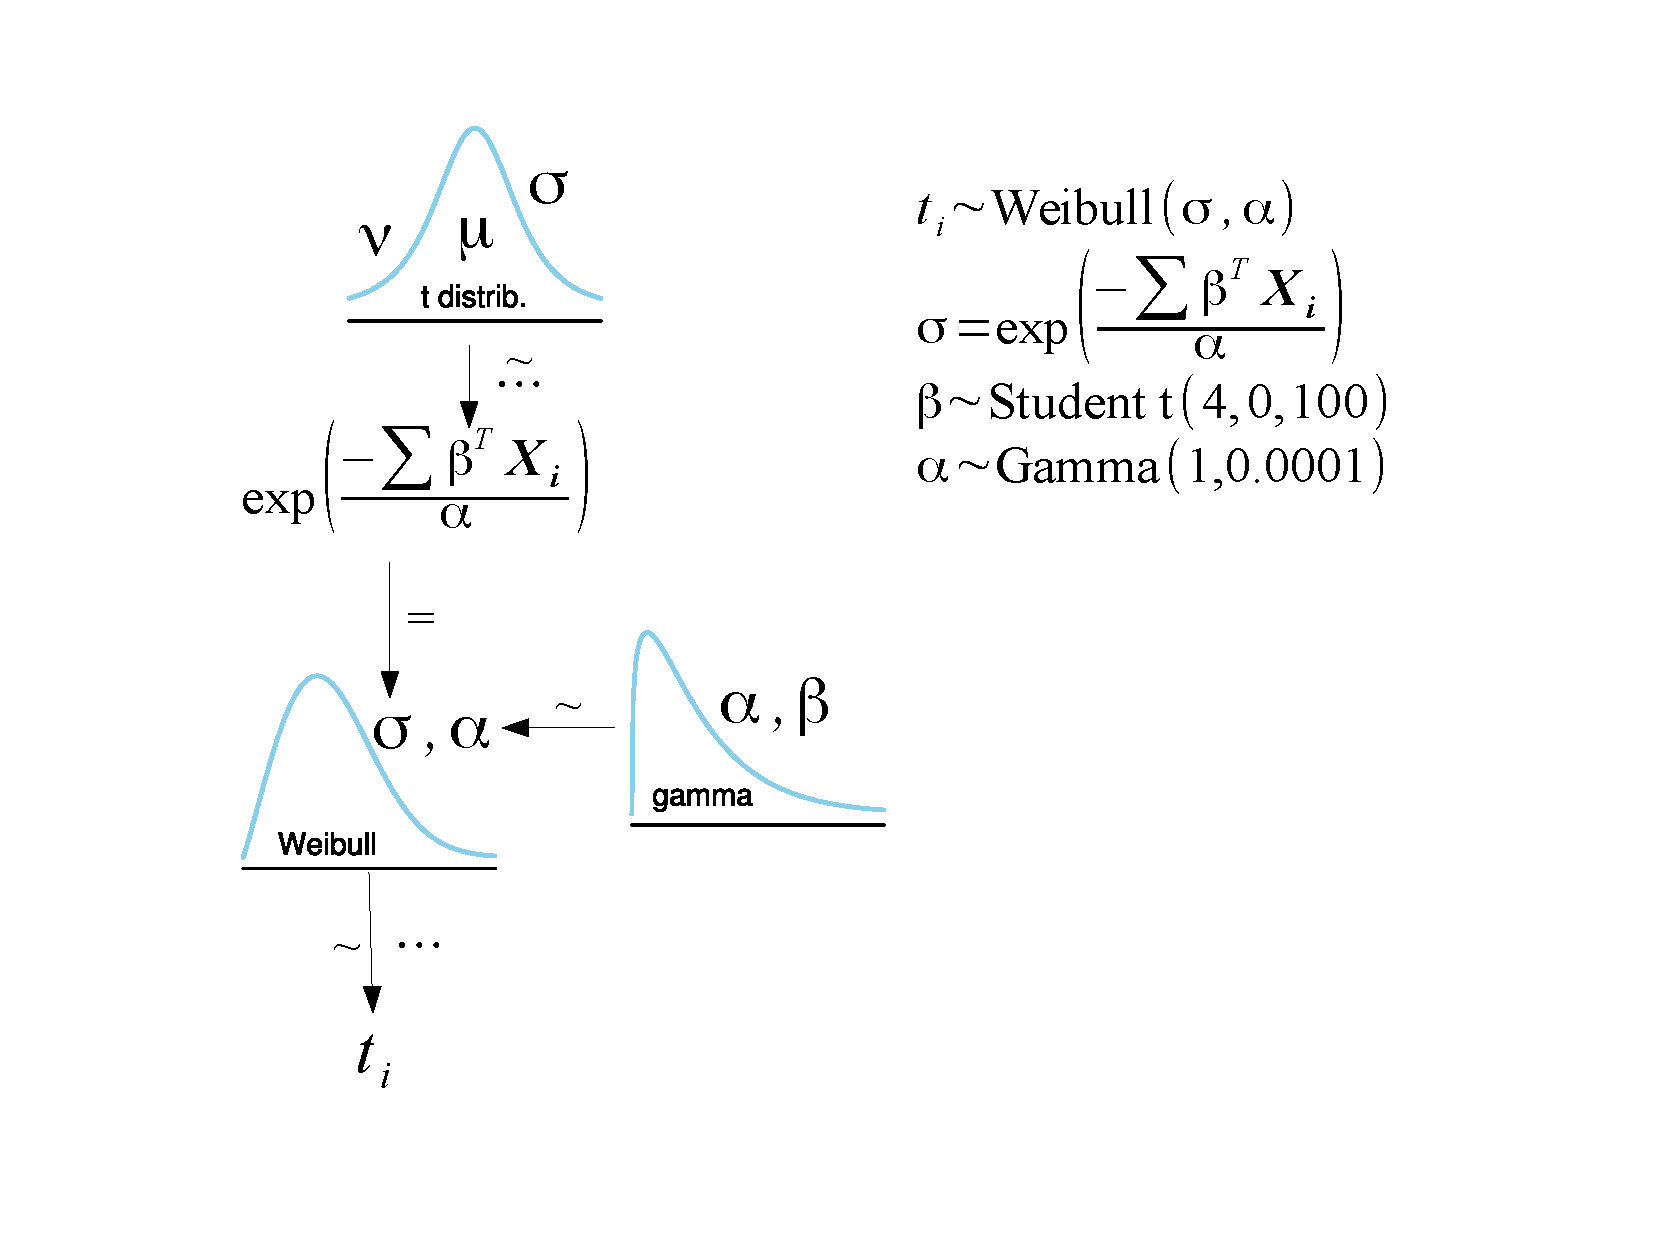
\includegraphics[height = 0.8\textheight, width = \textwidth,  keepaspectratio = true]{figure/brac_surv_mod}
  \end{center}
\end{frame}

\begin{frame}
  \frametitle{Current results\dots}
  \begin{center}
    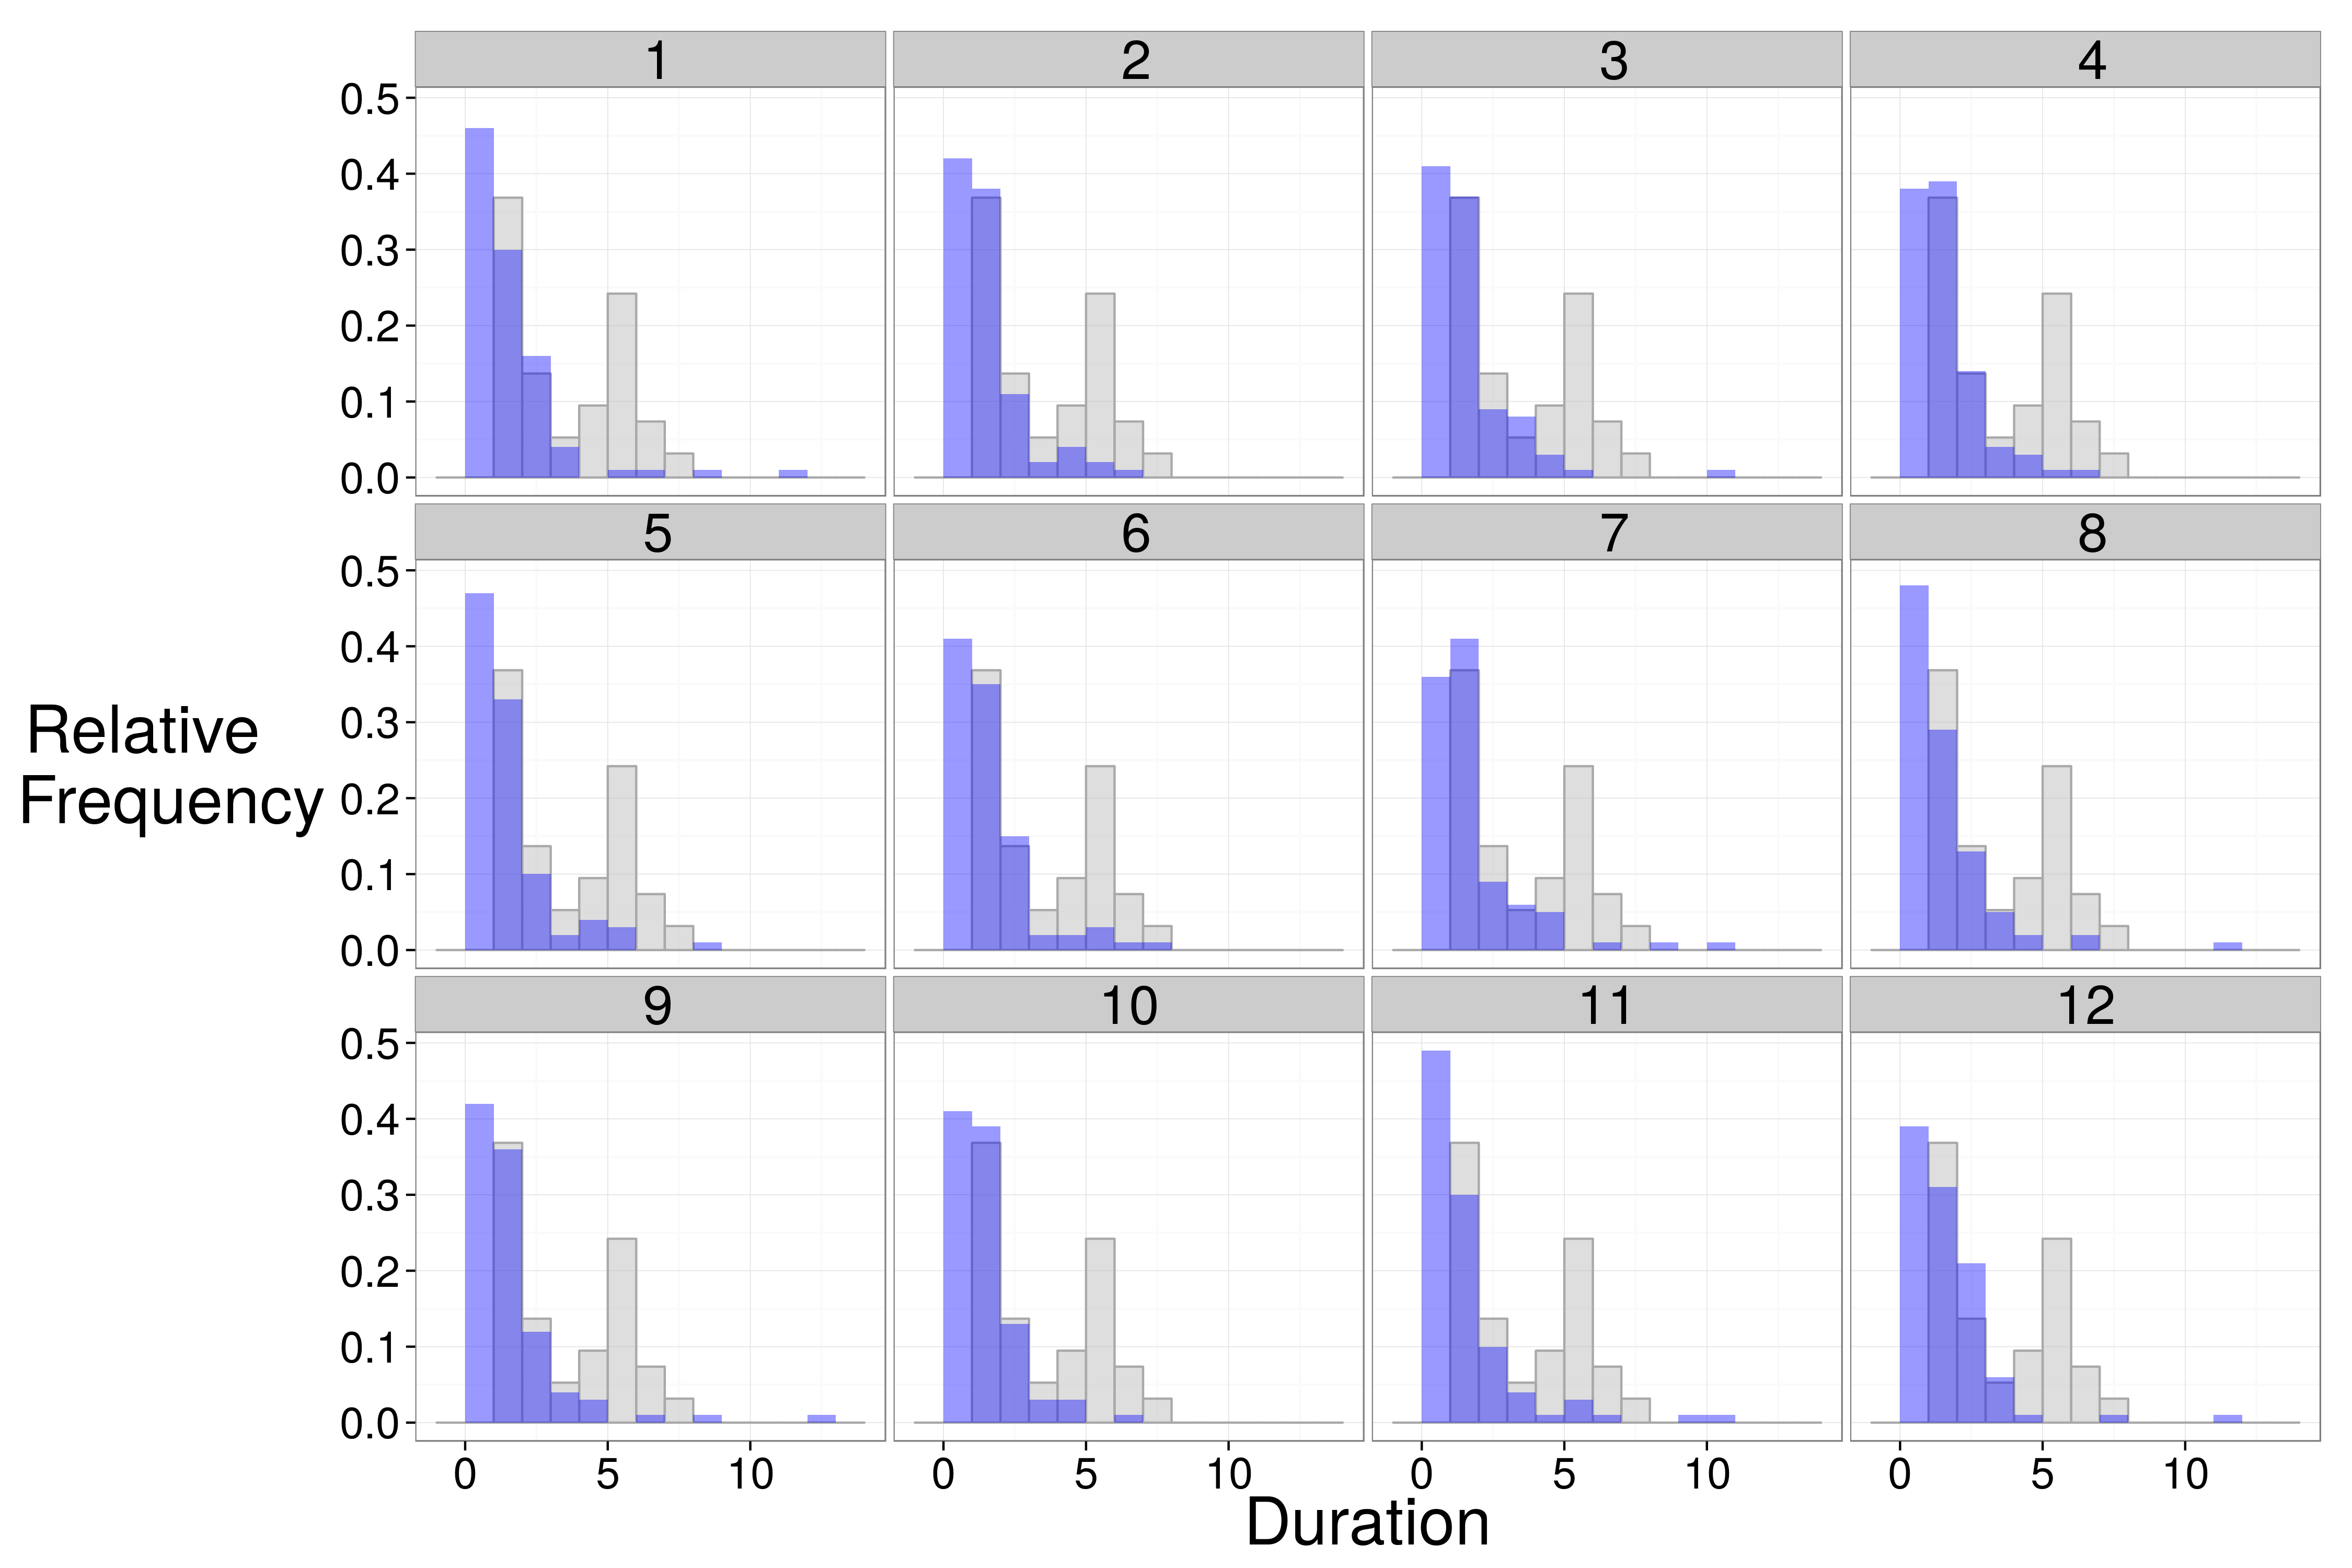
\includegraphics[height = 0.8\textheight, width = \textwidth,  keepaspectratio = true]{figure/brac_dur_post}
  \end{center}
\end{frame}

\begin{frame}
  \frametitle{Target and developing survival model}
  \begin{center}
    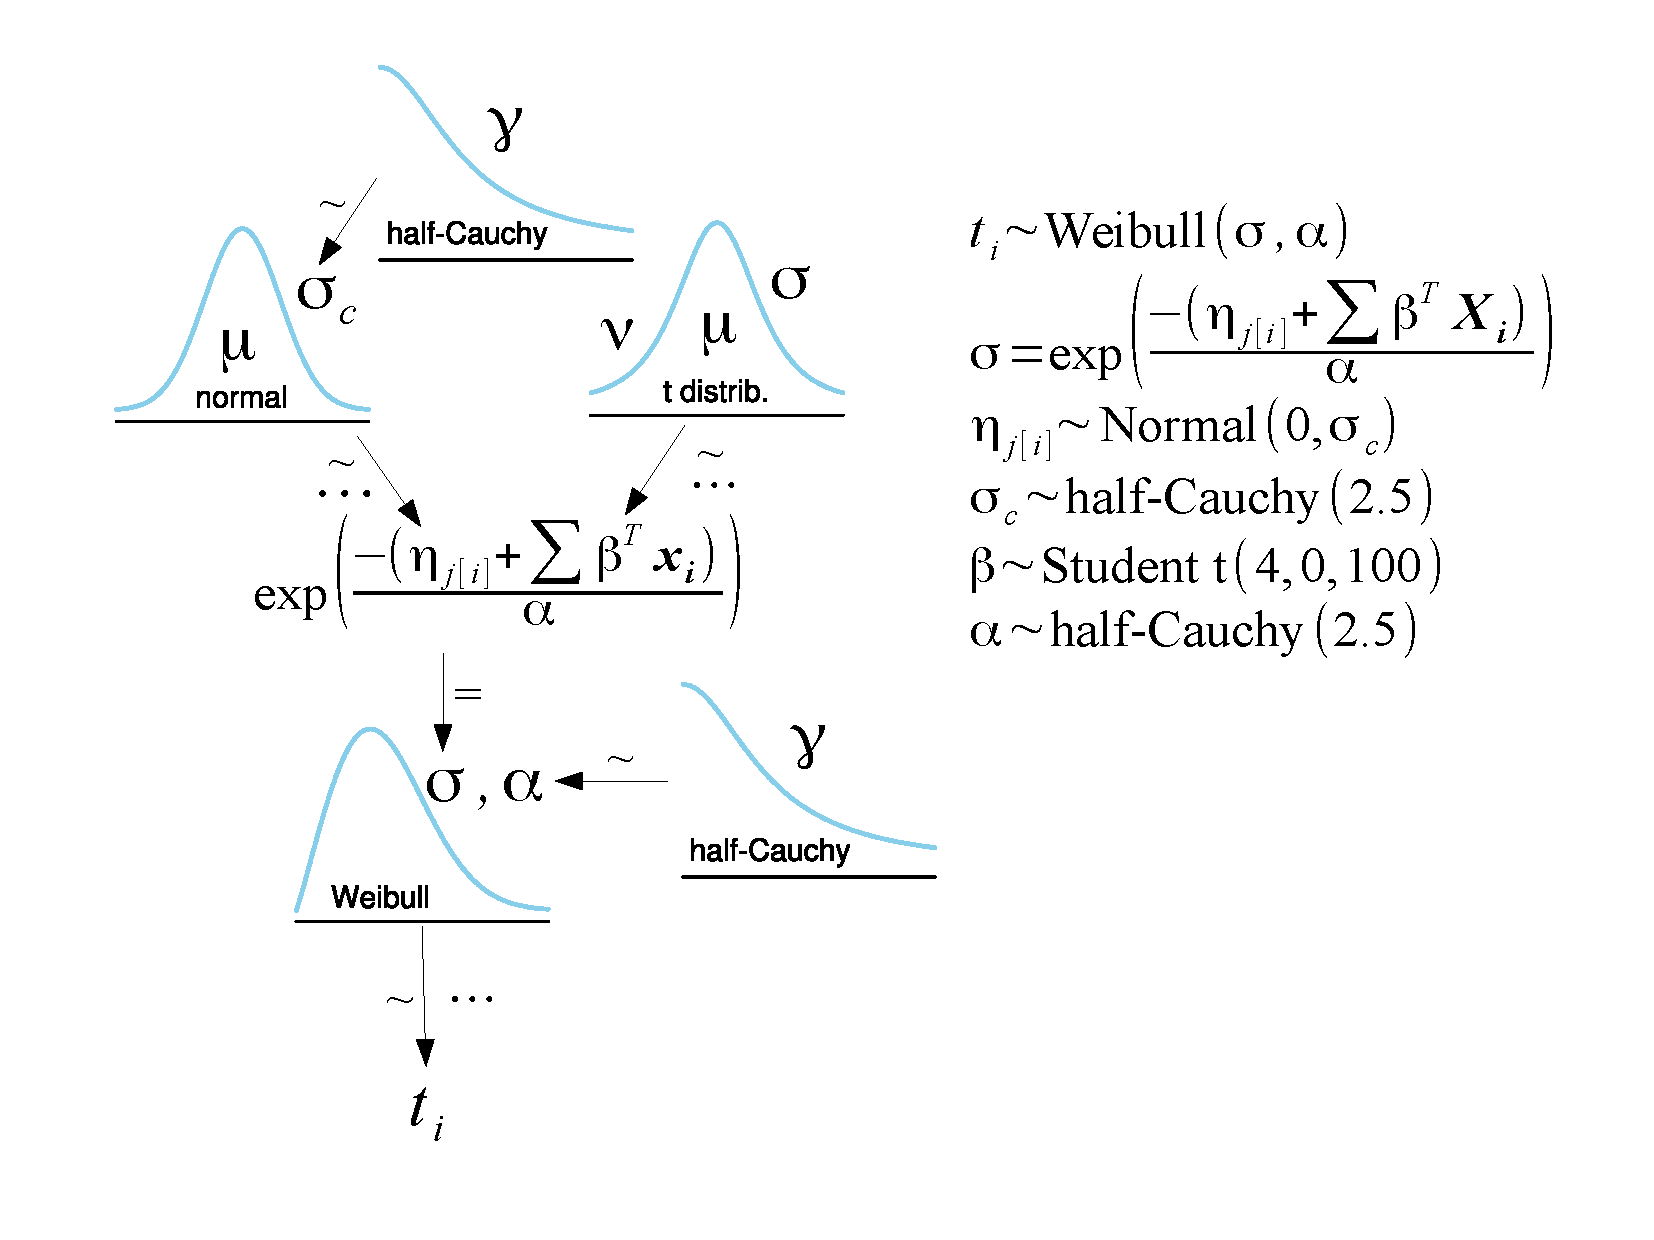
\includegraphics[height = 0.8\textheight, width = \textwidth,  keepaspectratio = true]{figure/brac_surv_mod_update}
  \end{center}
\end{frame}

\begin{frame}
  \frametitle{Point/counting process of fossils occurrence}

  A fossil is a count; number of fossils in temporal window.

  Hierarchical Poisson model of absolute sighting rate.

\end{frame}


\section{Mammals}
\begin{frame}
  Death and Taxa: biological, temporal, and historical effects on mammal species duration
\end{frame}

\begin{frame}
  \frametitle{North American survival}
  \begin{columns}
    \begin{column}{0.5\textwidth}
      \begin{itemize}
        \item species duration as measure of survival
        \item traits
          \begin{itemize}
            \item organismal: diet, locomotor categories
            \item species: body size, bioprovince occupancy
          \end{itemize}
        \item origination cohort
        \item phylogeny primarily based on taxonomy
      \end{itemize}
    \end{column}
    \begin{column}{0.5\textwidth}
      \begin{itemize}
        \item duration defined as number of 2My bins from FAD to LAD, inclusive
        \item fully Bayesian hierarchical model
        \item censoring approach
          \begin{itemize}
            \item if still extant, right censored
            \item if not extant and duration of only 1 bin, left censored
          \end{itemize}
      \end{itemize}
    \end{column}
  \end{columns}
\end{frame}

\begin{frame}
  \frametitle{Model diagram}
  \begin{center}
    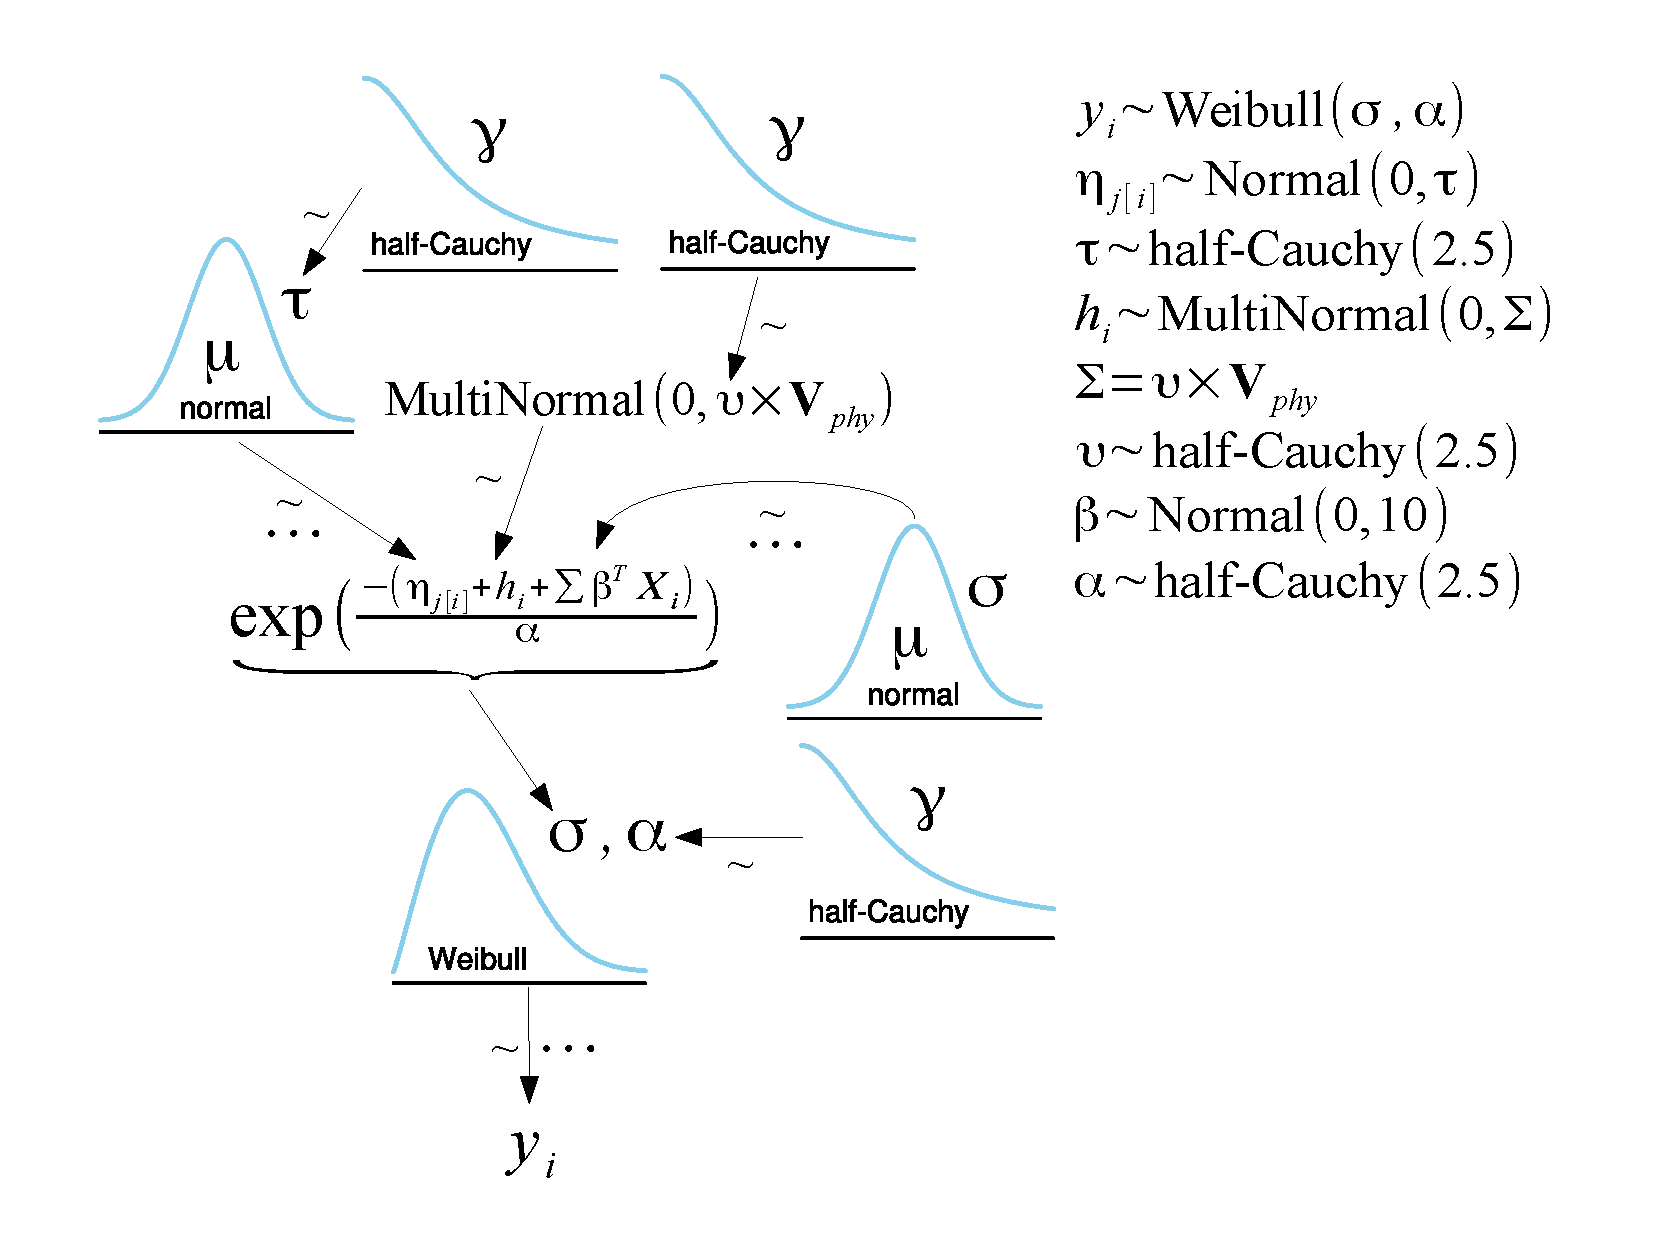
\includegraphics[height = 0.8\textheight, width = \textwidth,  keepaspectratio = true]{figure/mammal_survival_model}
  \end{center}
\end{frame}

\begin{frame}
  \frametitle{Censoring}
  \begin{center}
    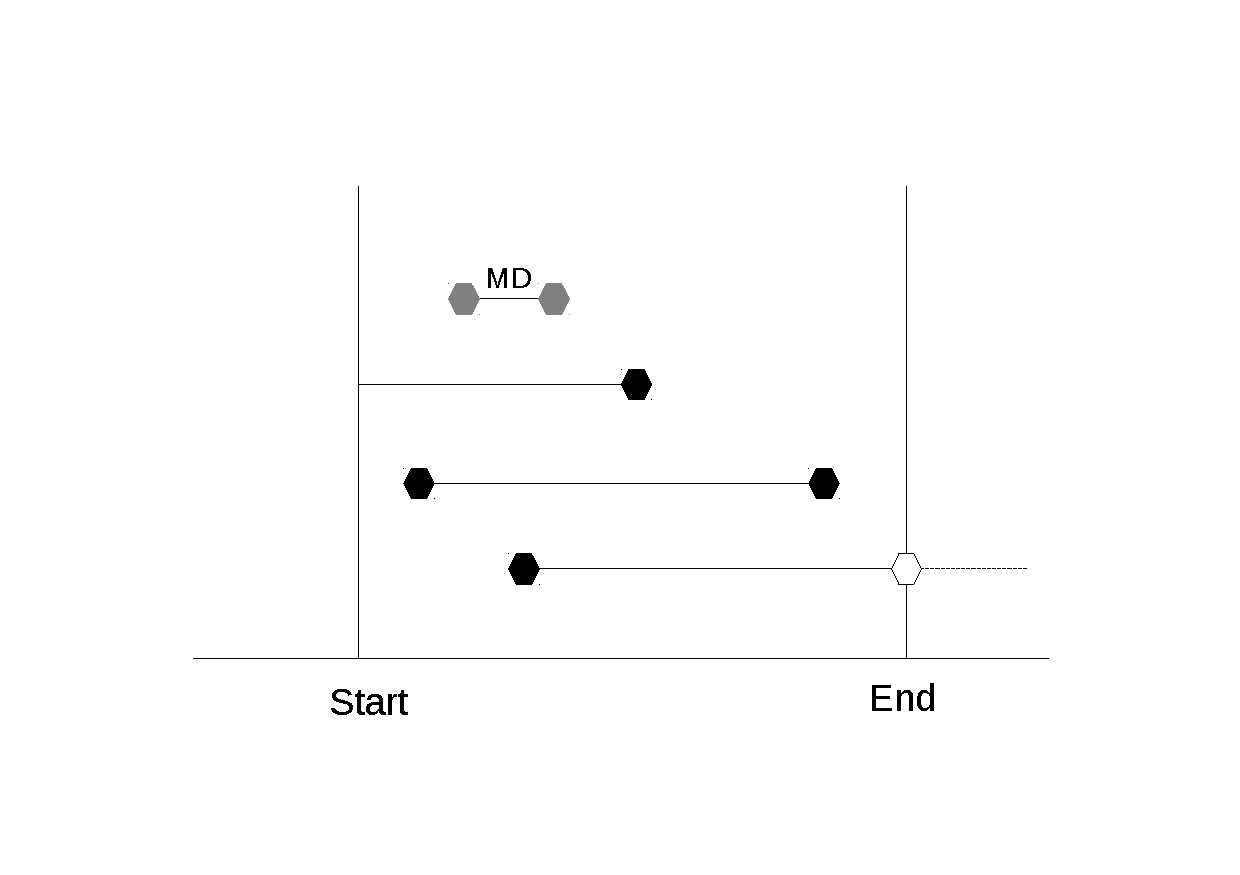
\includegraphics[height = 0.8\textheight, width = \textwidth,  keepaspectratio = true]{figure/censoring_diagram}
  \end{center}
\end{frame}

\begin{frame}
  \frametitle{Modeling censored observations}
  \begin{definition}
    \(S(t | \alpha, \sigma) = \exp\left(-\left(\frac{t}{\sigma}\right)^{\alpha}\right)\)
  \end{definition}

  Right censored evaluated at \(S(t)\), left at \(1 - S(t)\). 
  
  Equivalent to ccdf and cdf respectively.
\end{frame}

\begin{frame}
  \frametitle{Modeling censored observations}
  \begin{block}{Likelihood}
    \(L \propto \prod_{i \in C} \mathrm{Weibull}(y_{i} | \alpha, \sigma) \prod_{j \in R} S(y_j | \alpha, \sigma) \prod_{k \in L} \left(1 - S(y_{k} | \alpha, \sigma)\right)\)
  \end{block}

\end{frame}

\begin{frame}
  \frametitle{Posterior predictive checks: S(t)}
  \begin{center}
    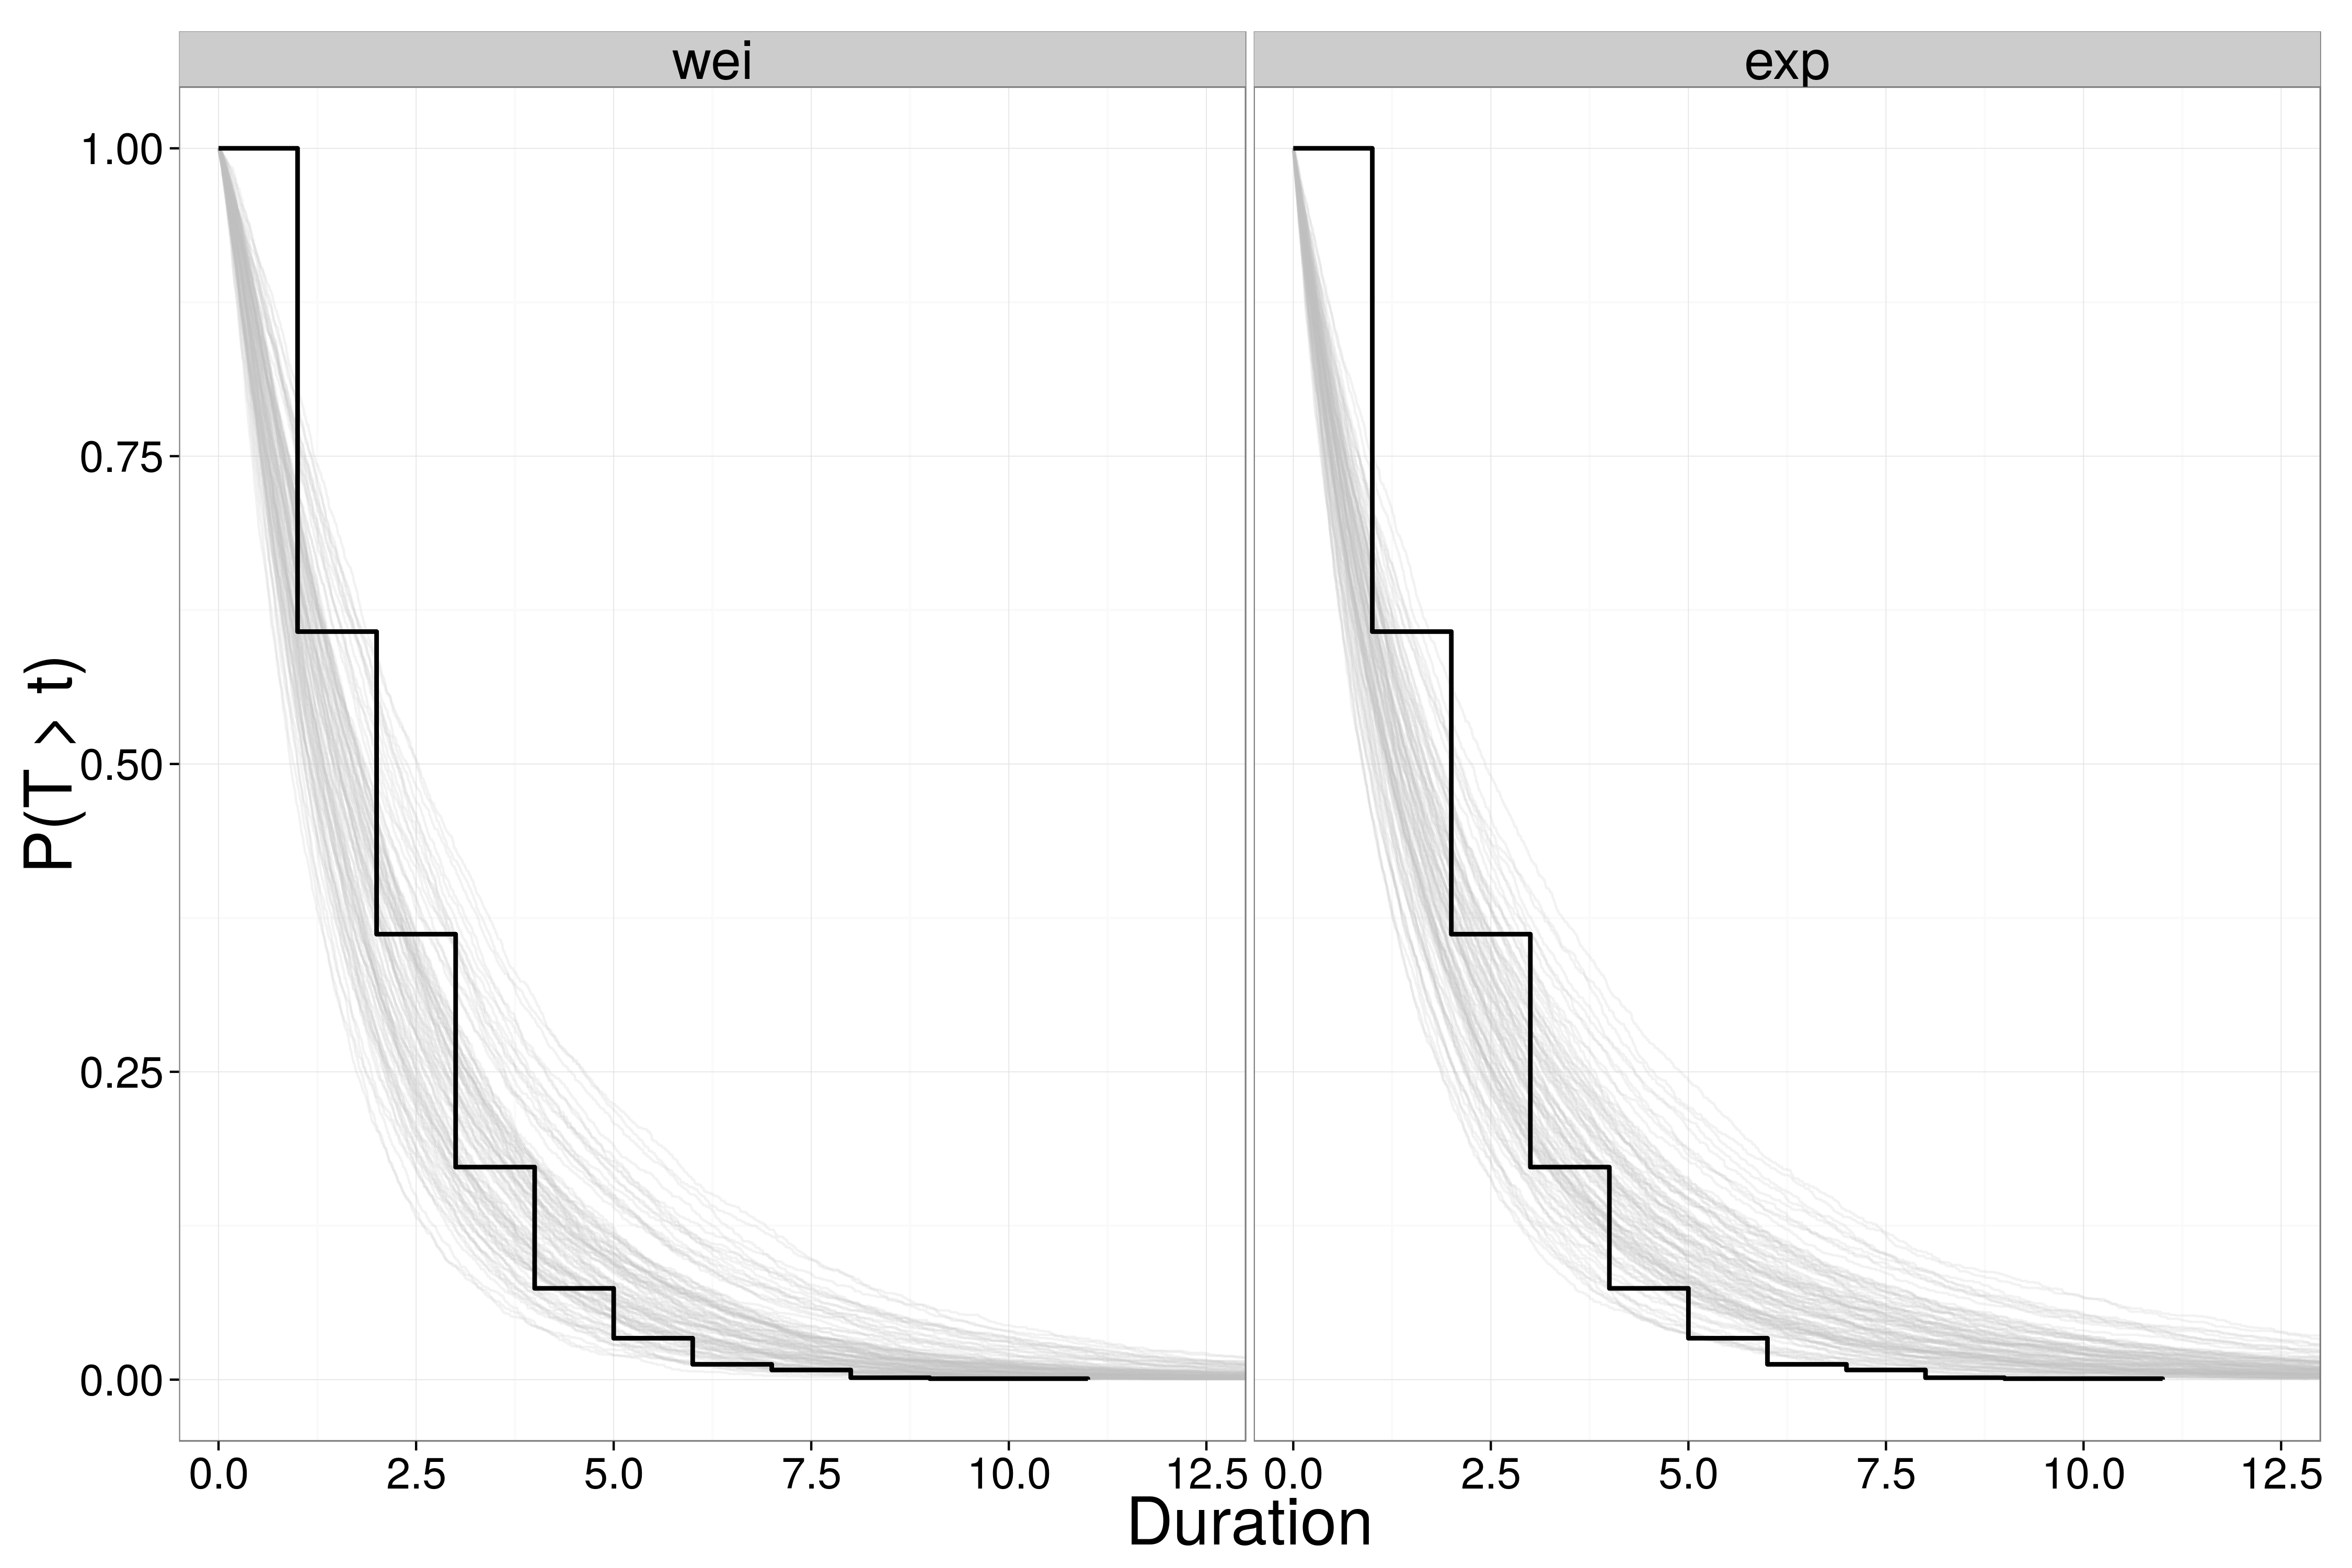
\includegraphics[height = 0.8\textheight, width = \textwidth,  keepaspectratio = true]{figure/survival_function}
  \end{center}
\end{frame}

\begin{frame}
  \frametitle{Posterior predictive checks: deviance residuals}
  \begin{center}
    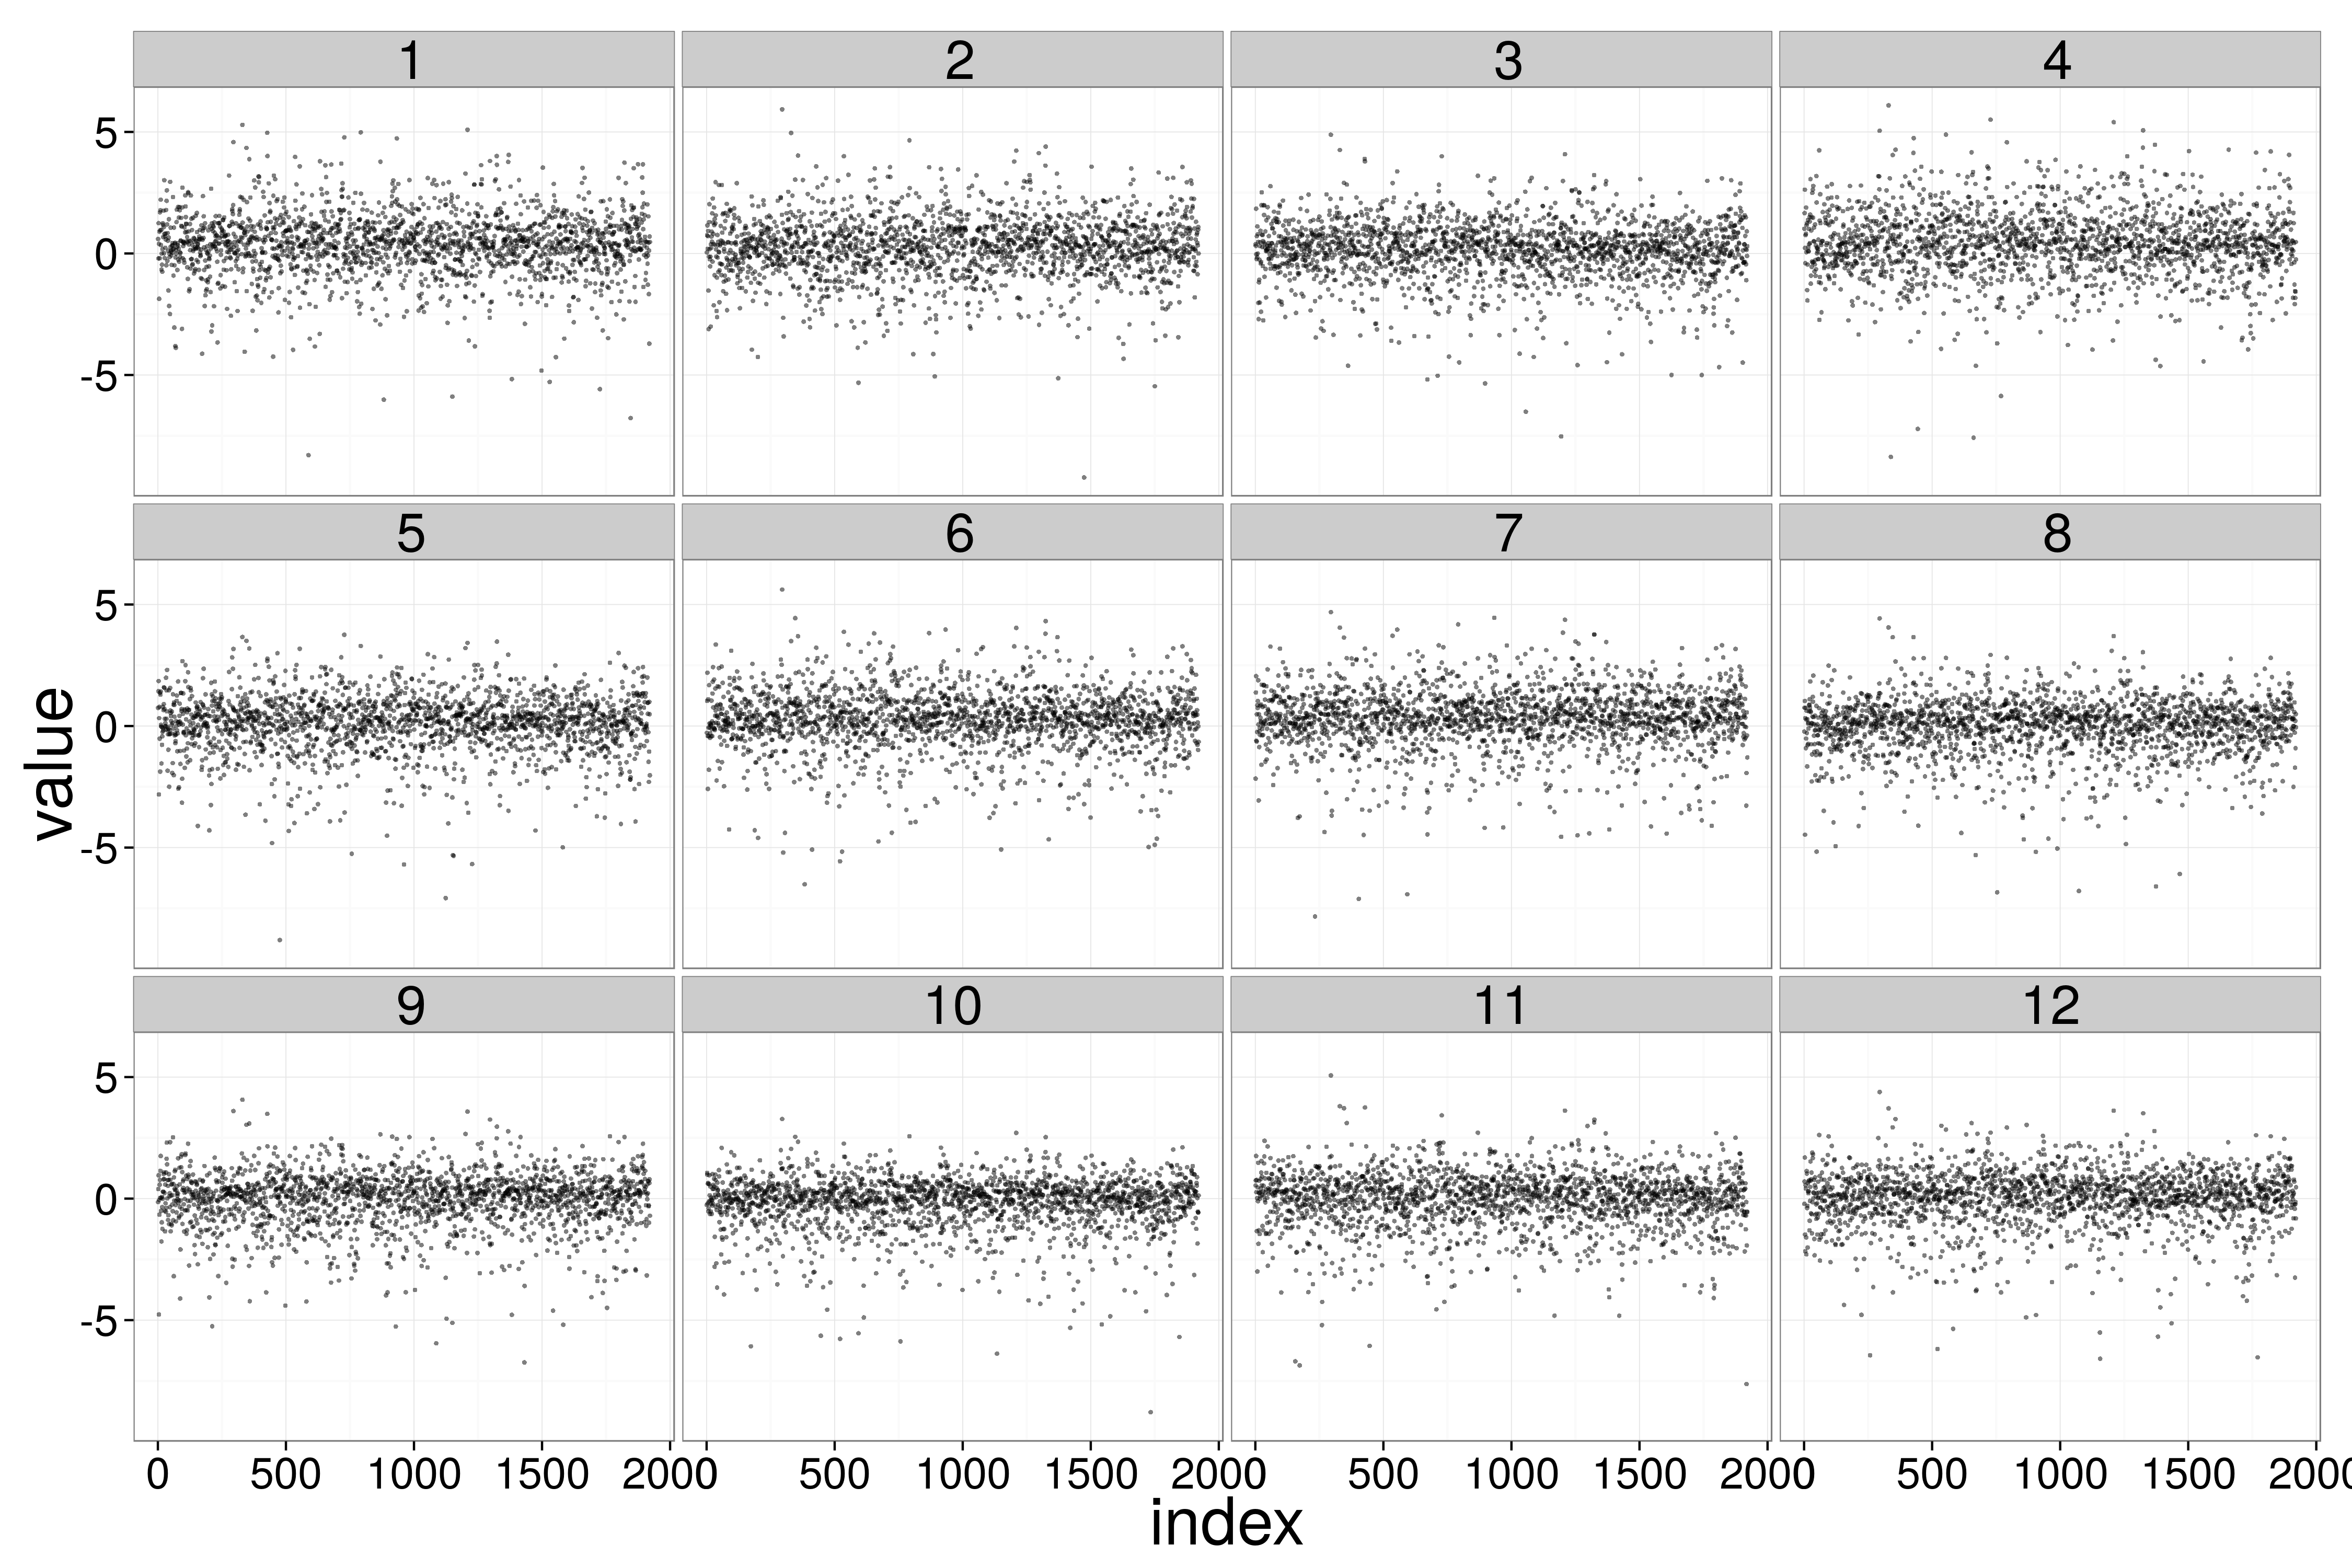
\includegraphics[height = 0.8\textheight, width = \textwidth,  keepaspectratio = true]{figure/residual_plot}
  \end{center}
\end{frame}

\begin{frame}
  \frametitle{Posterior predictive checks: point checks}
  \begin{center}
    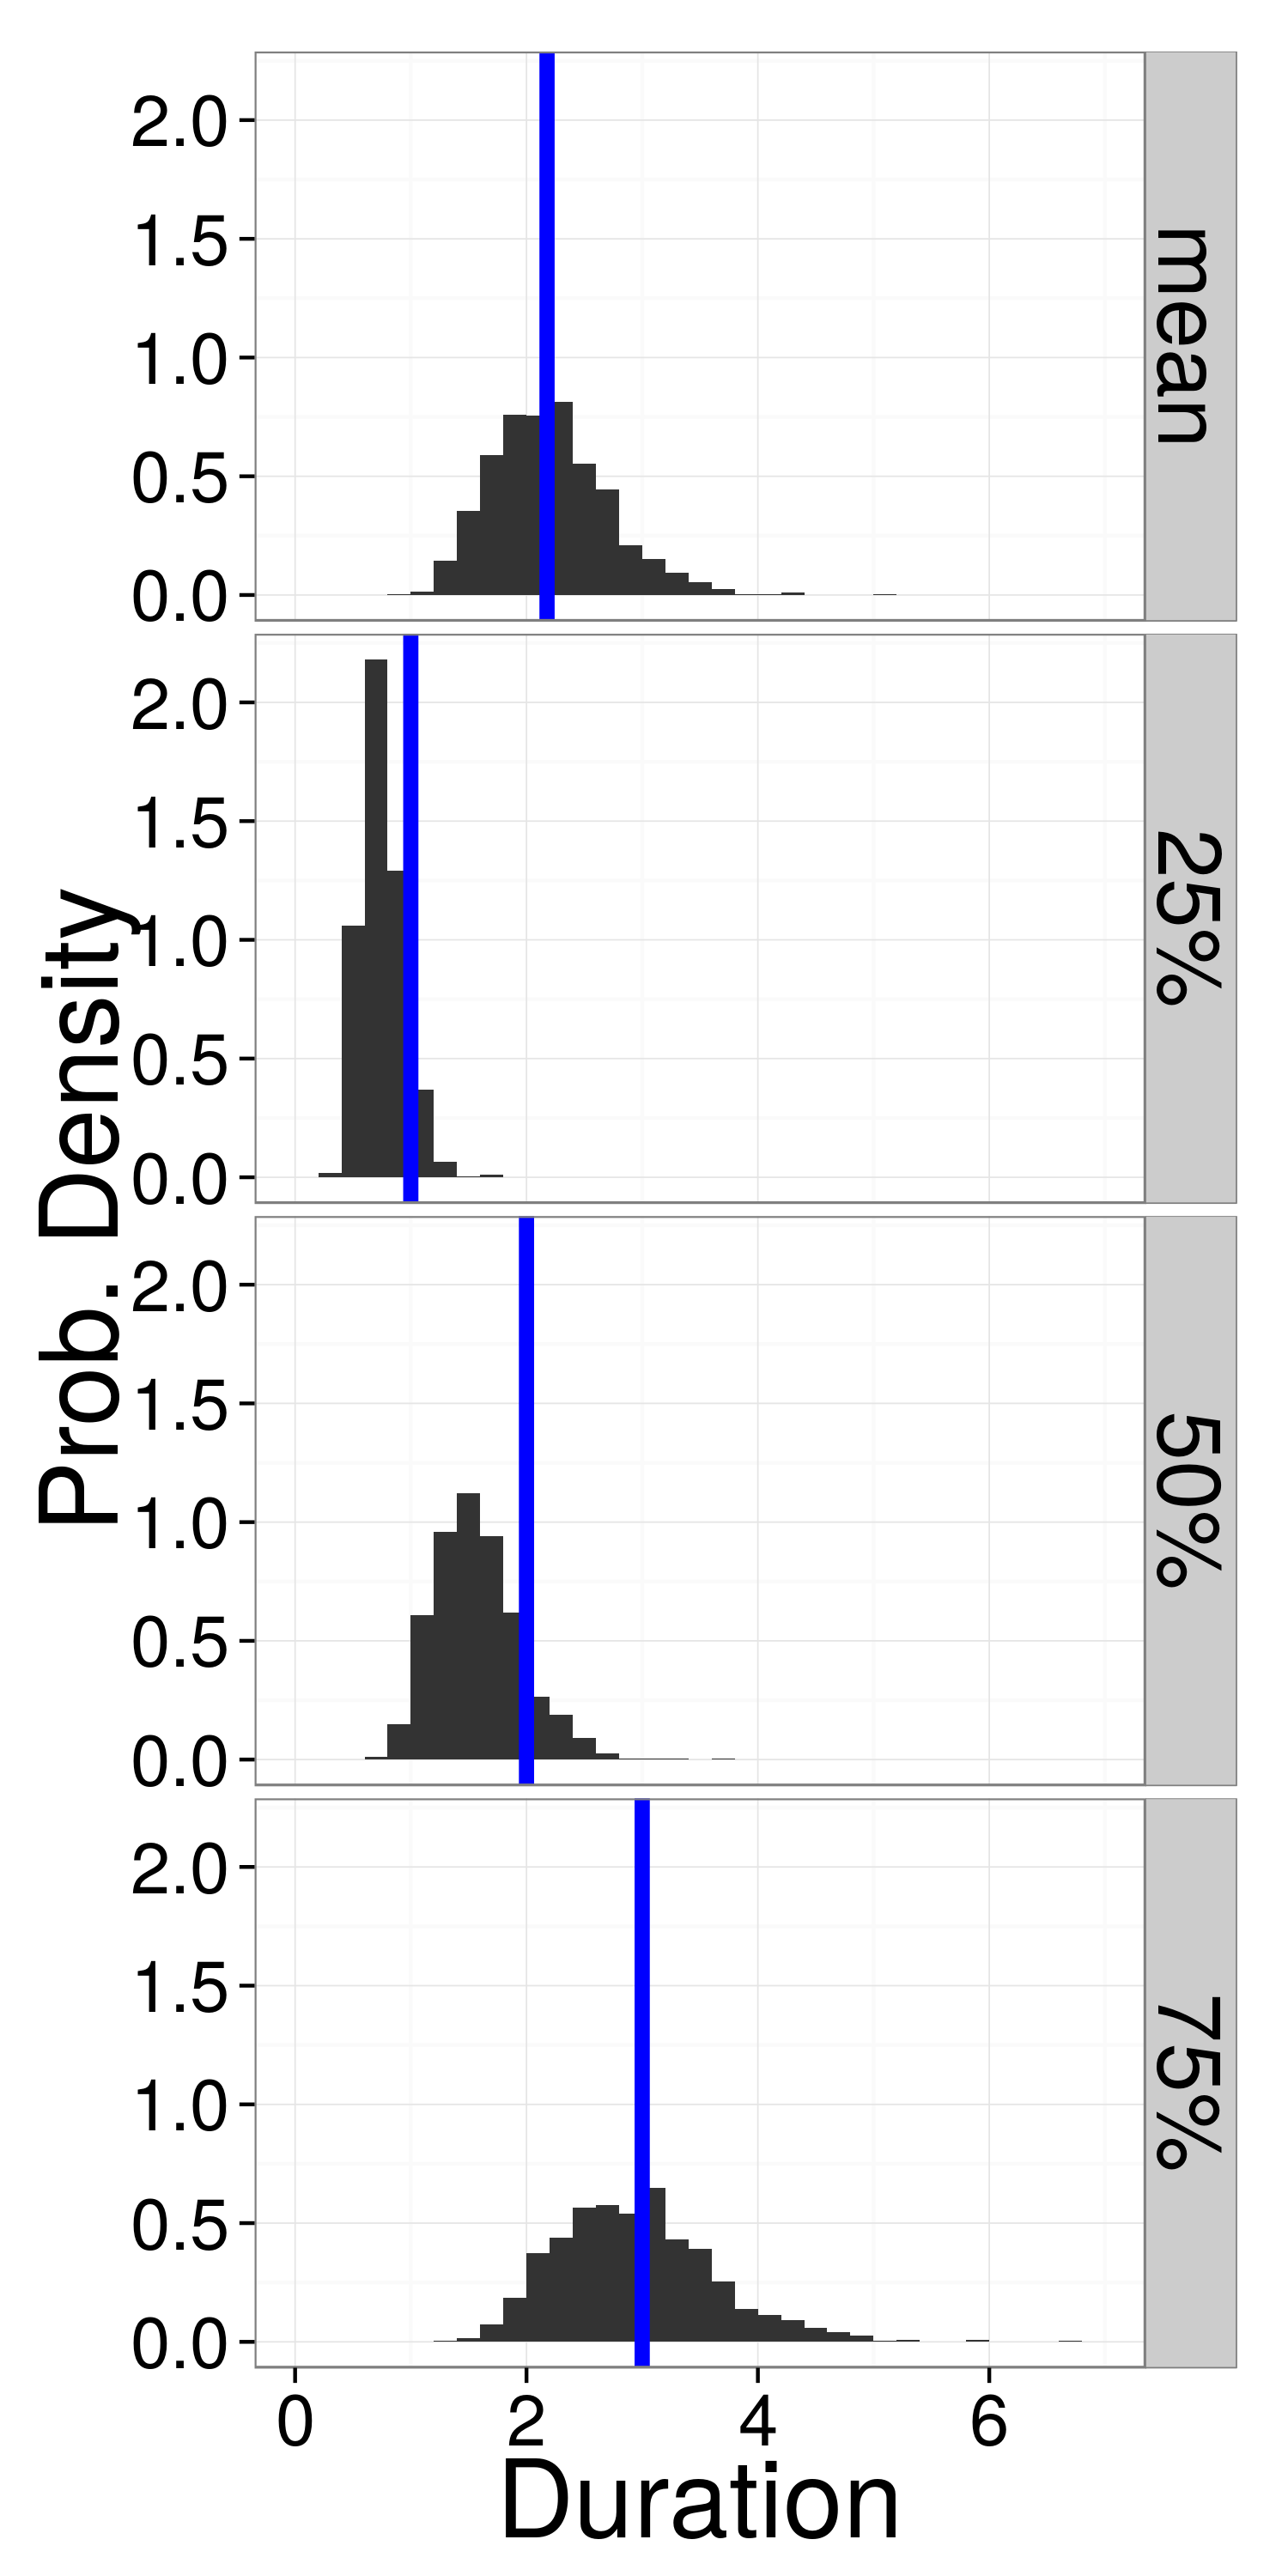
\includegraphics[height = 0.8\textheight, width = \textwidth,  keepaspectratio = true]{figure/quant_ppc}
  \end{center}
\end{frame}

\begin{frame}
  \frametitle{Pairwise differences of \(\beta\), dietary category}
  \begin{center}
    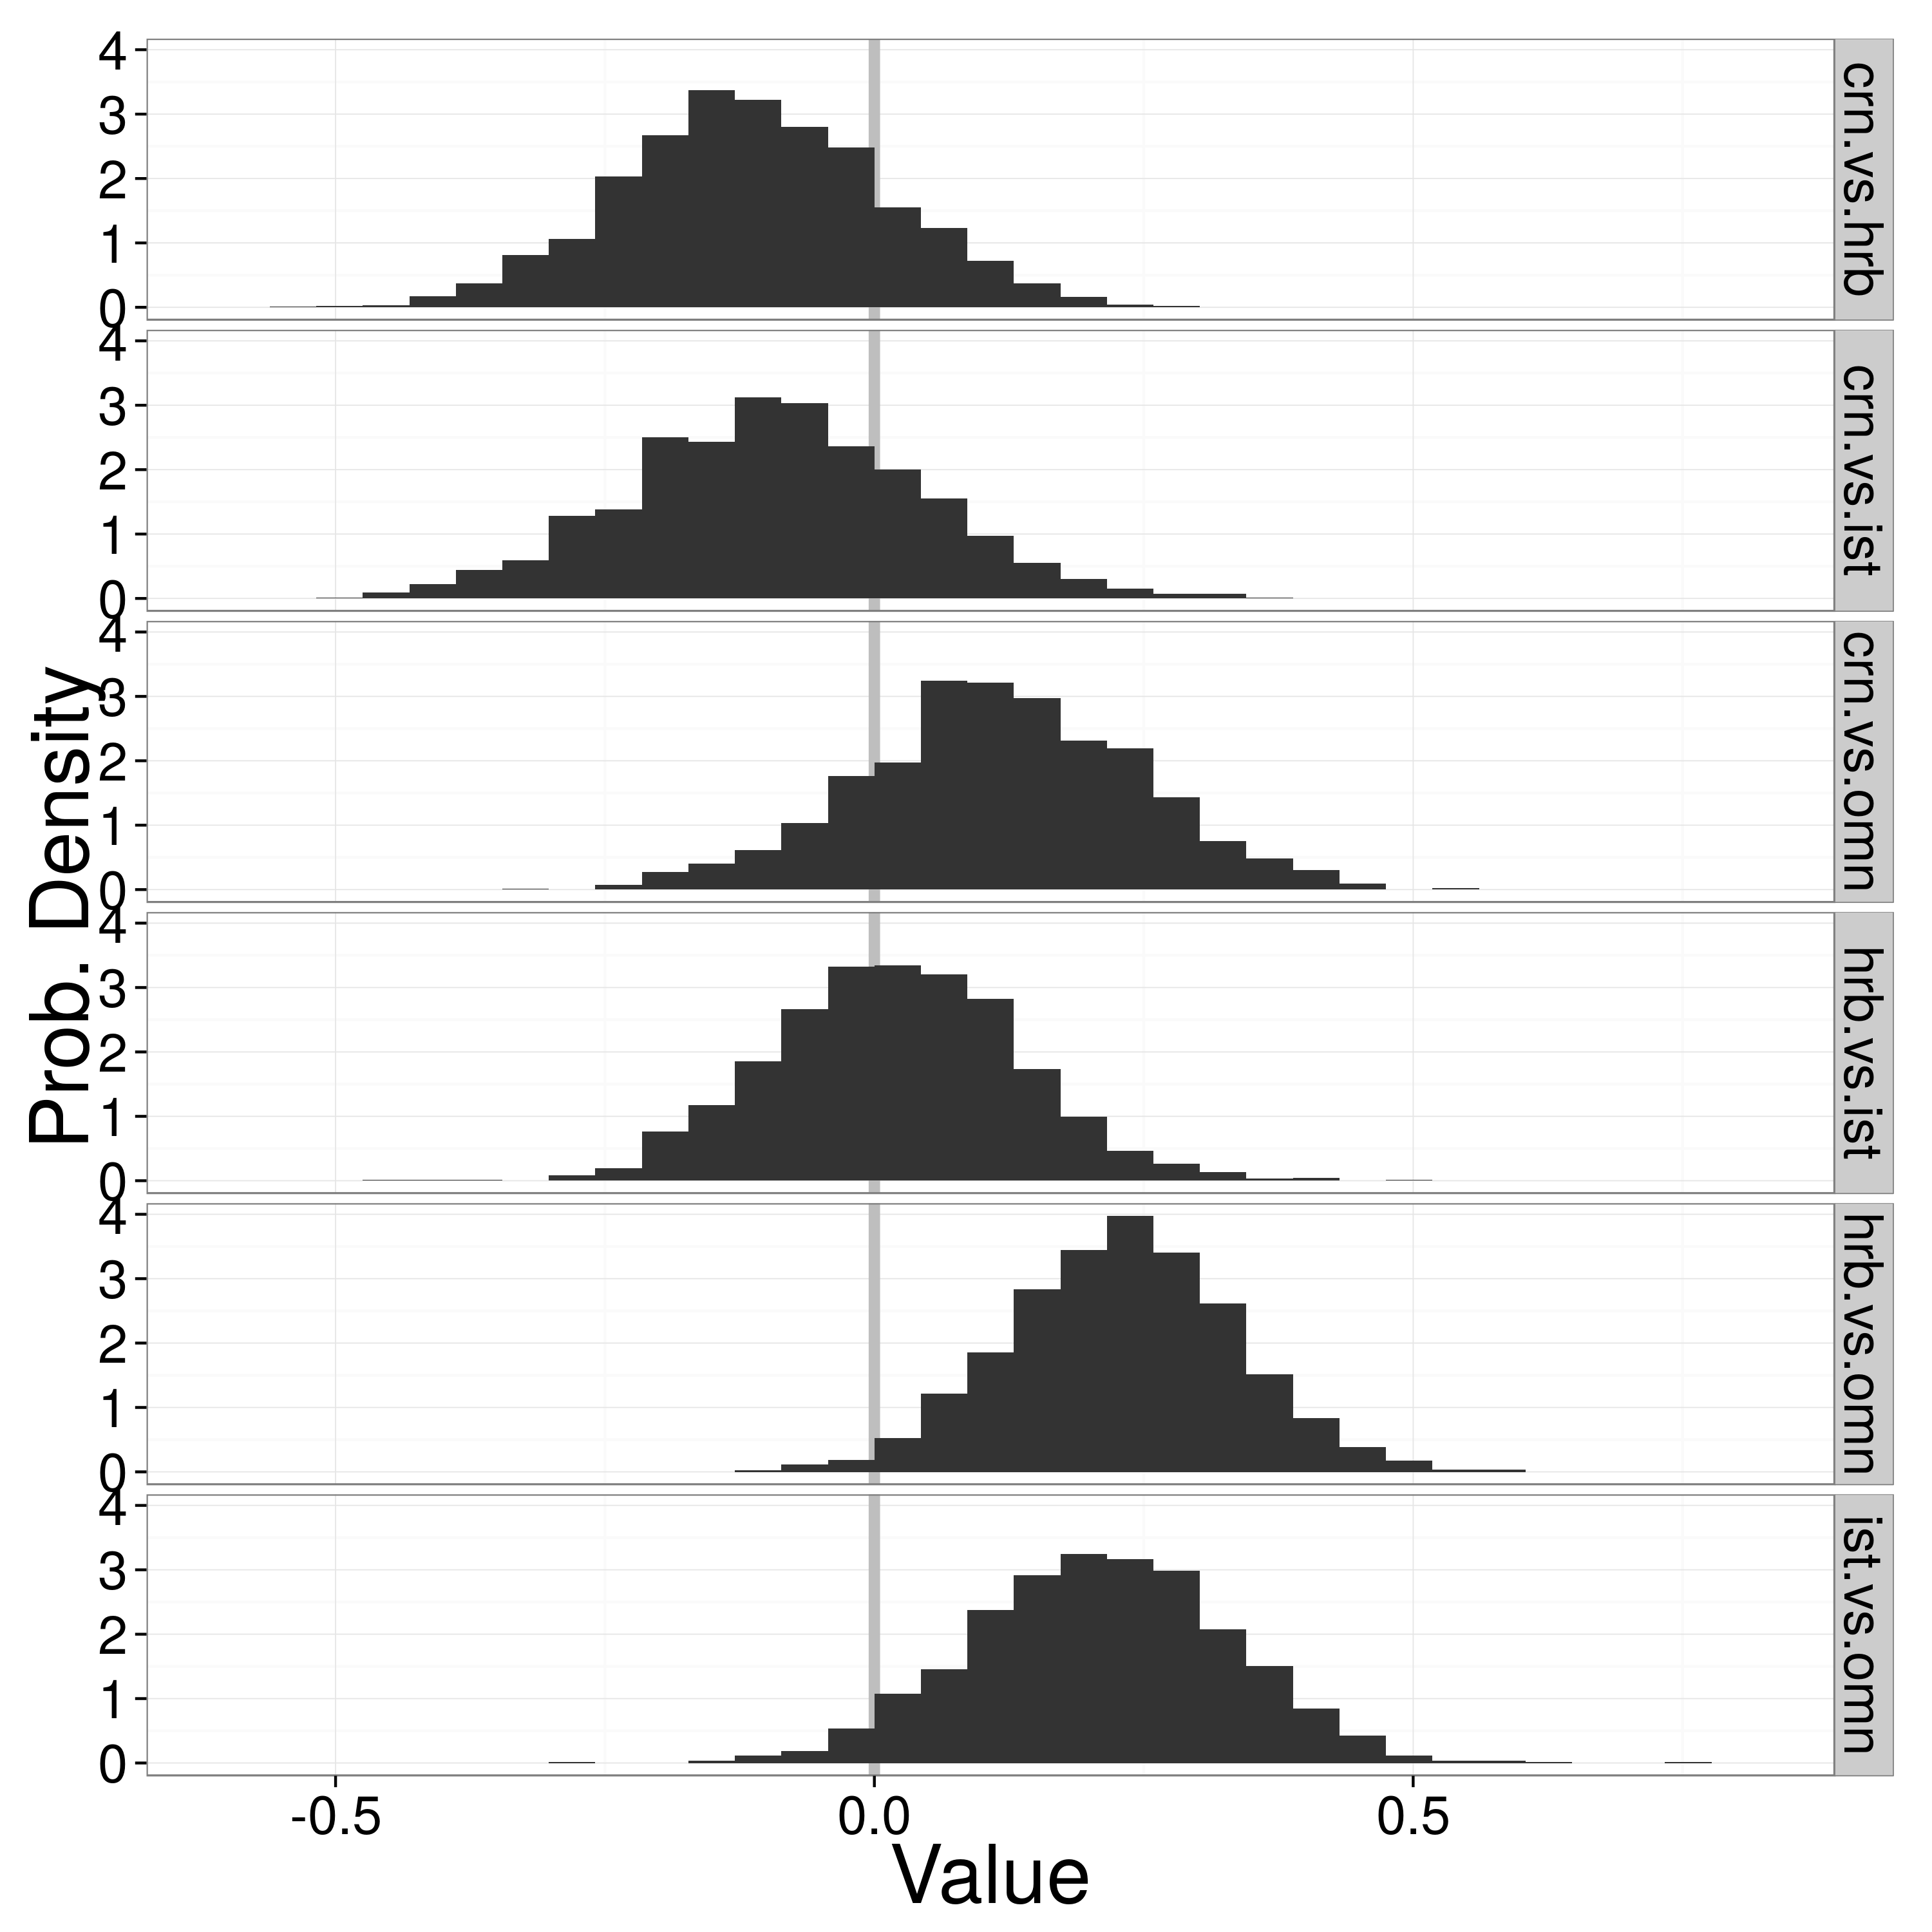
\includegraphics[height = 0.8\textheight, width = \textwidth,  keepaspectratio = true]{figure/diet_diff_est}
  \end{center}
\end{frame}

\begin{frame}
  \frametitle{Pairwise differences of \(\beta\), locomotor category}
  \begin{center}
    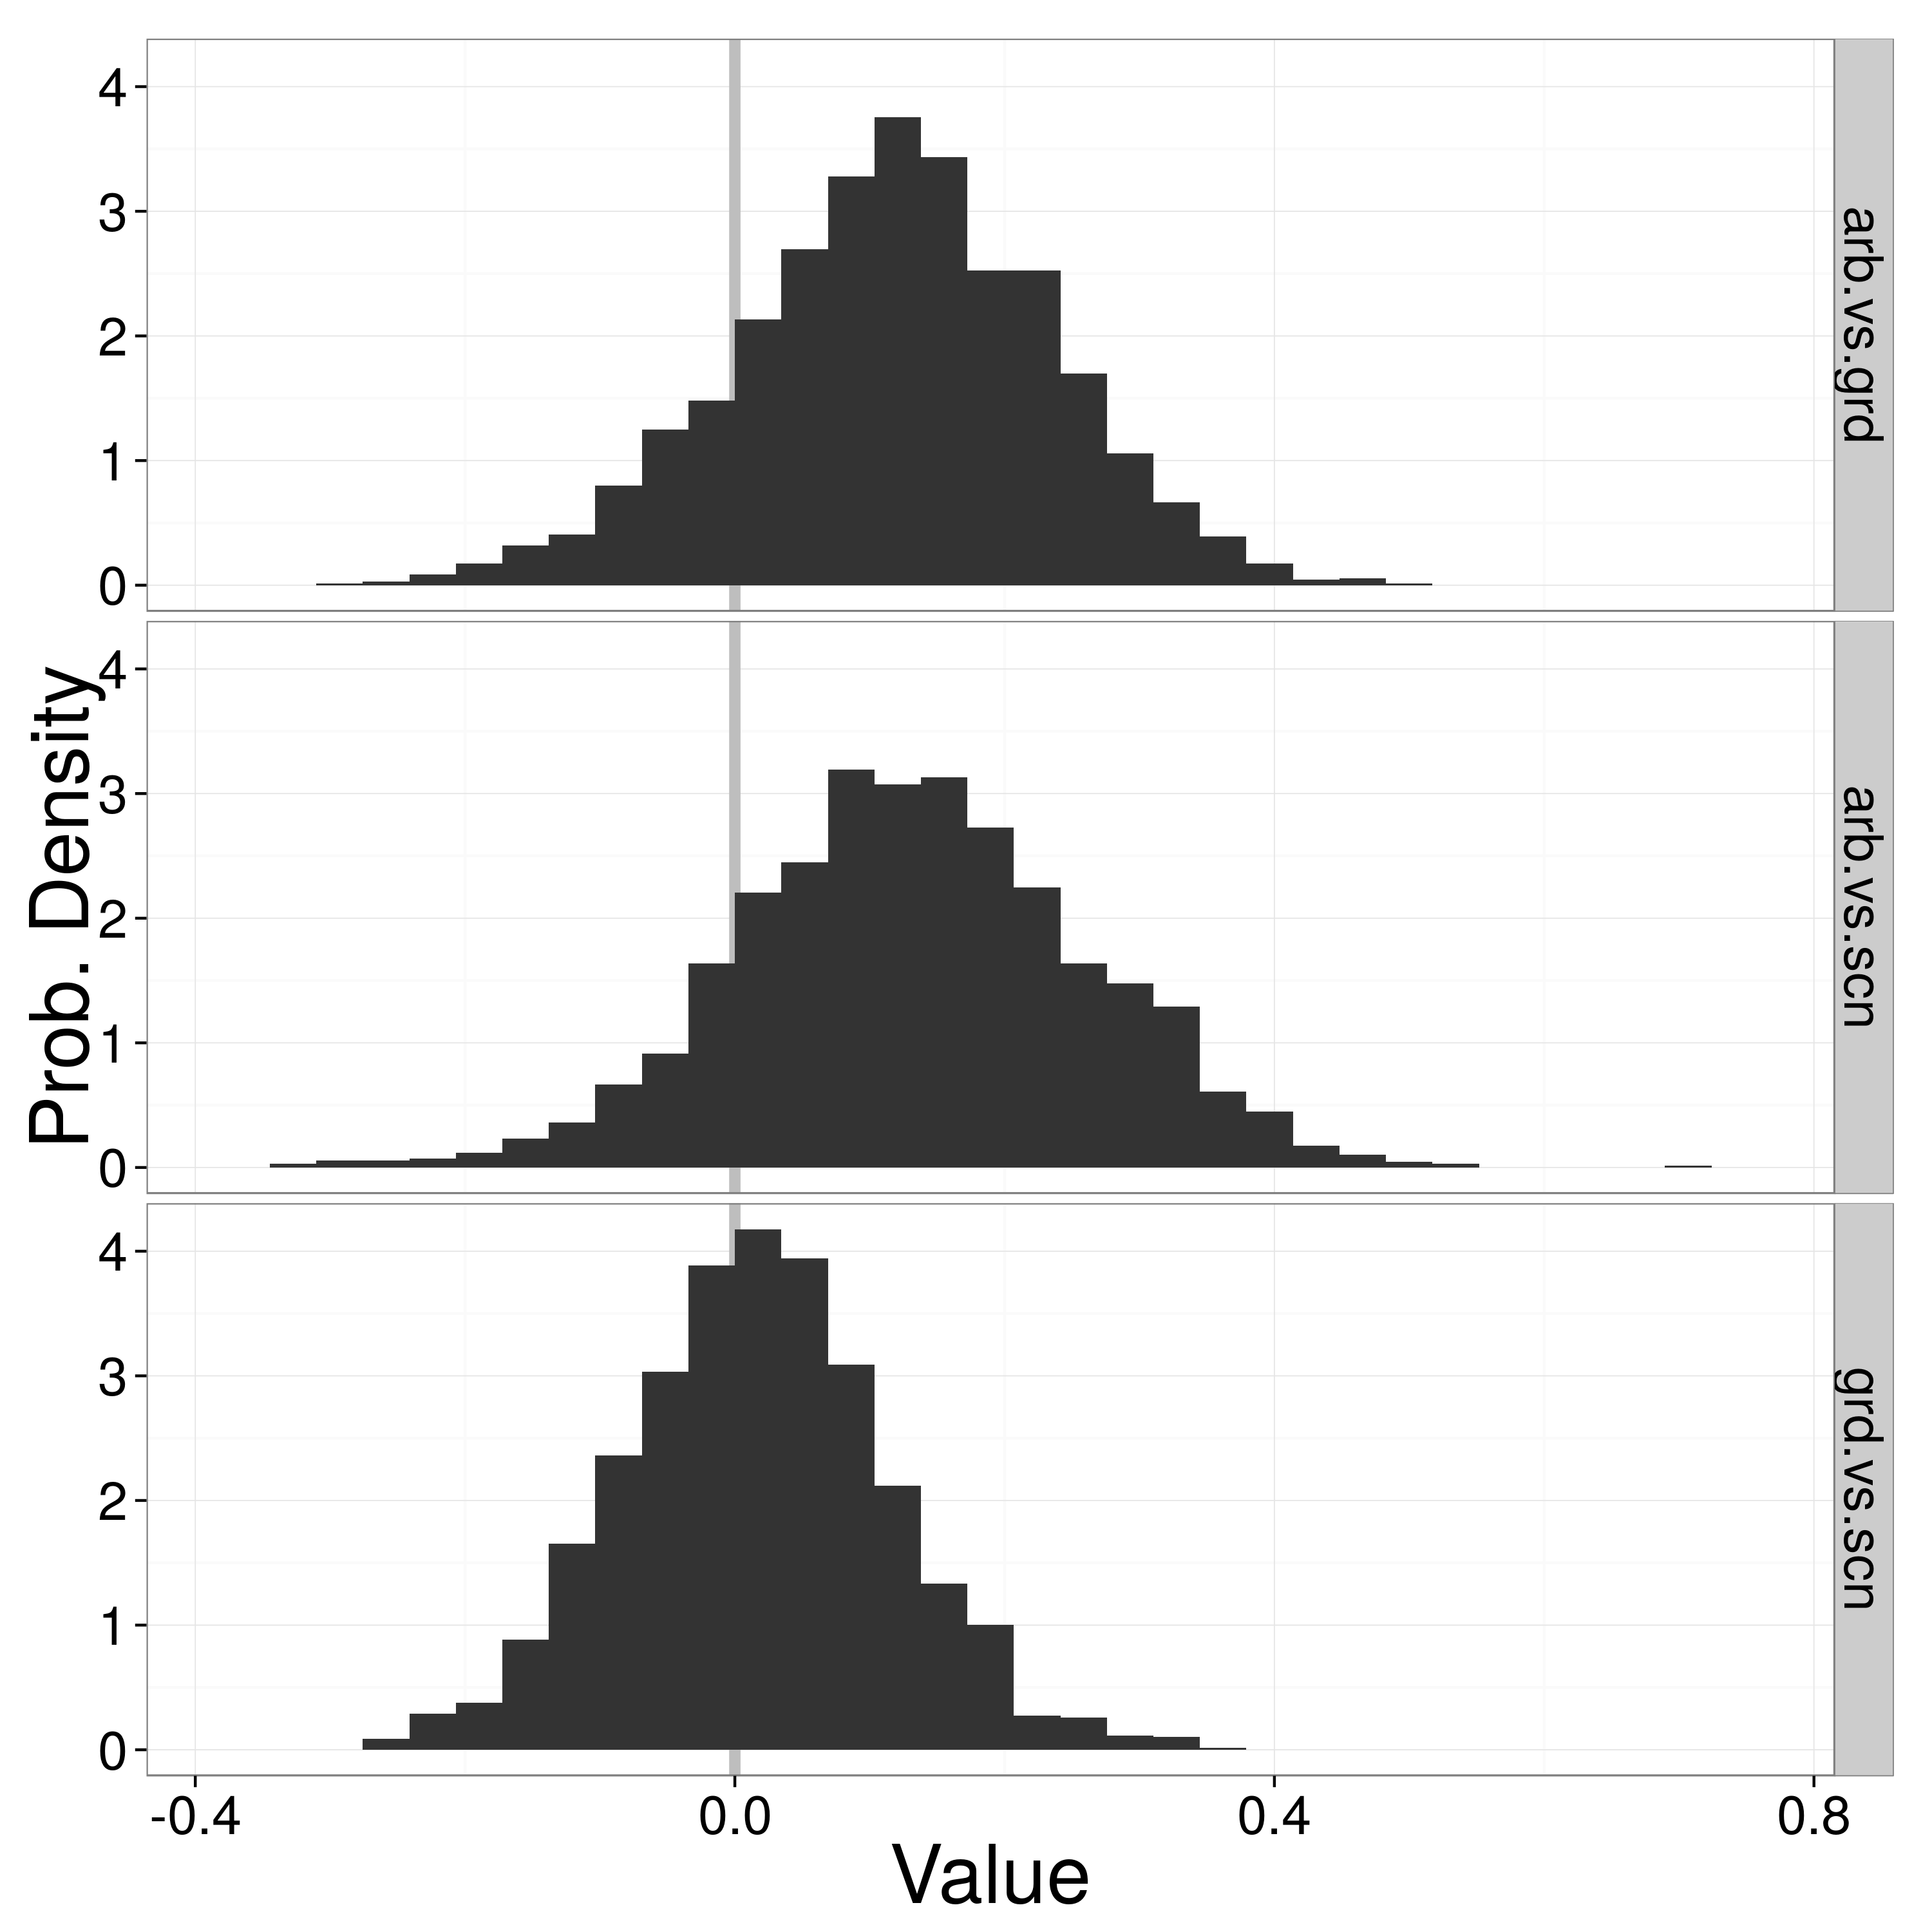
\includegraphics[height = 0.8\textheight, width = \textwidth,  keepaspectratio = true]{figure/loco_diff_est}
  \end{center}
\end{frame}

\begin{frame}
  \frametitle{Other traits}
  \begin{center}
    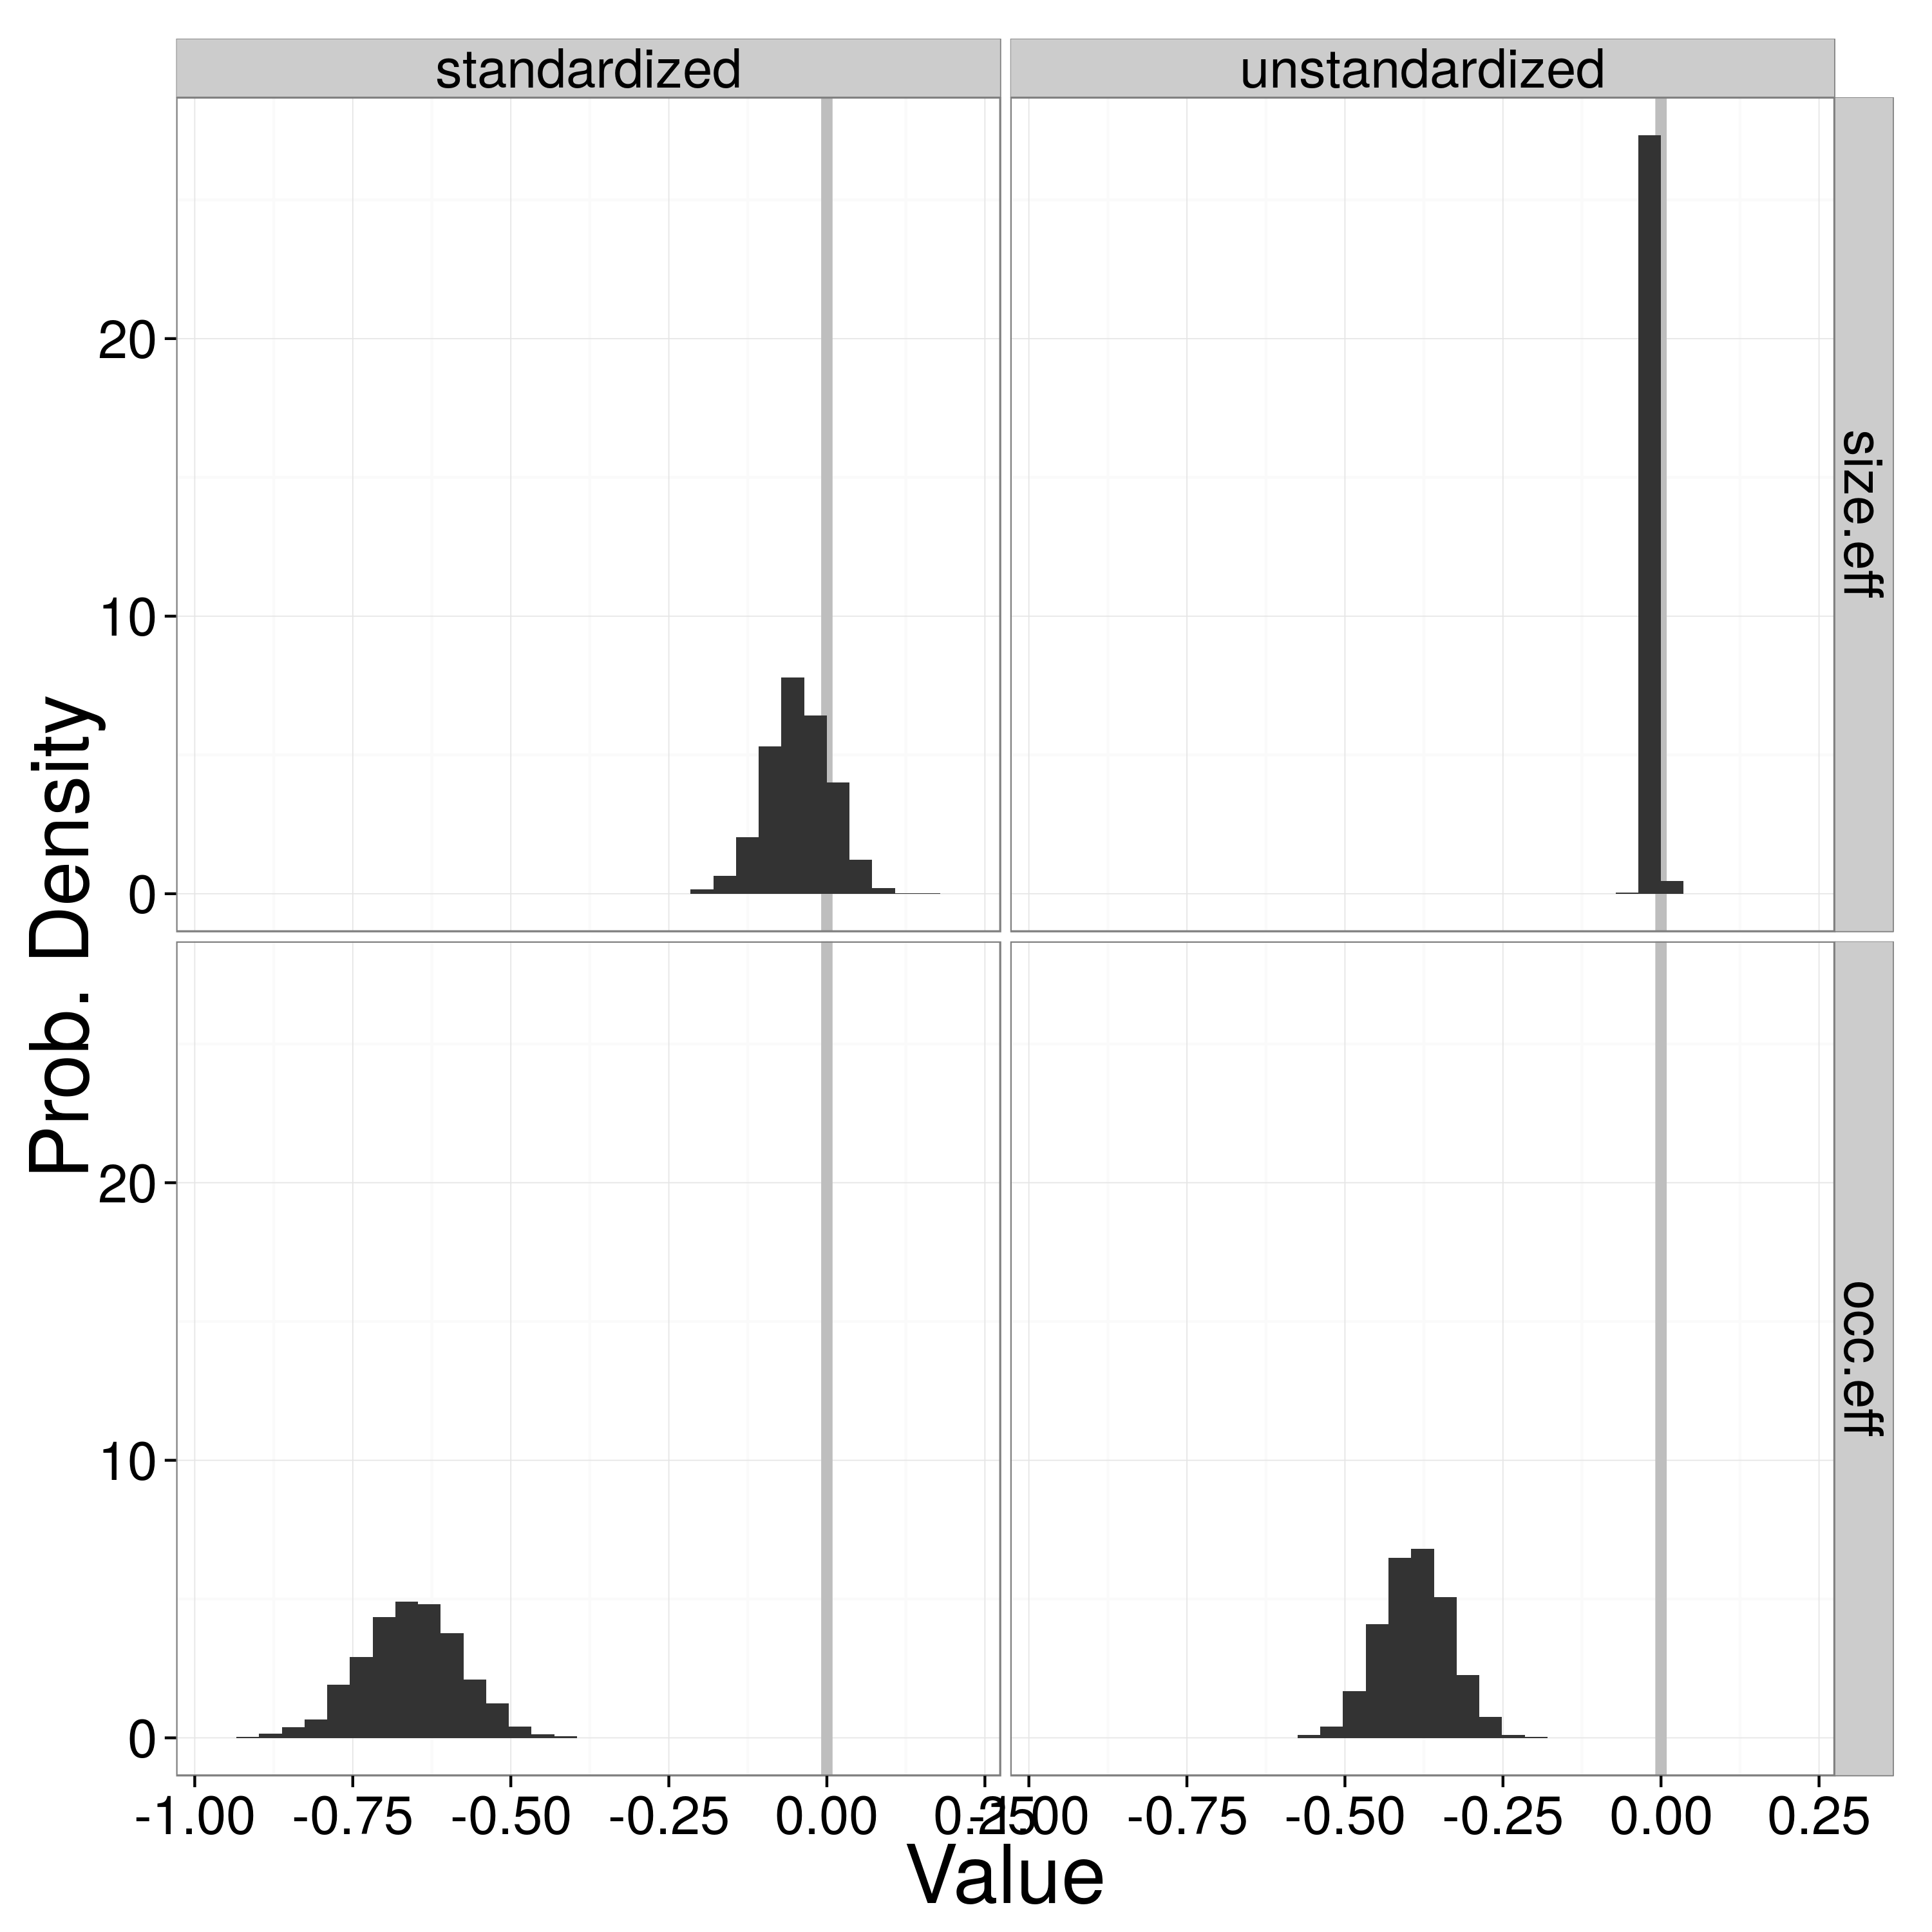
\includegraphics[height = 0.8\textheight, width = \textwidth,  keepaspectratio = true]{figure/other_est}
  \end{center}
\end{frame}

\begin{frame}
  \frametitle{Cohort effect}
  \begin{center}
    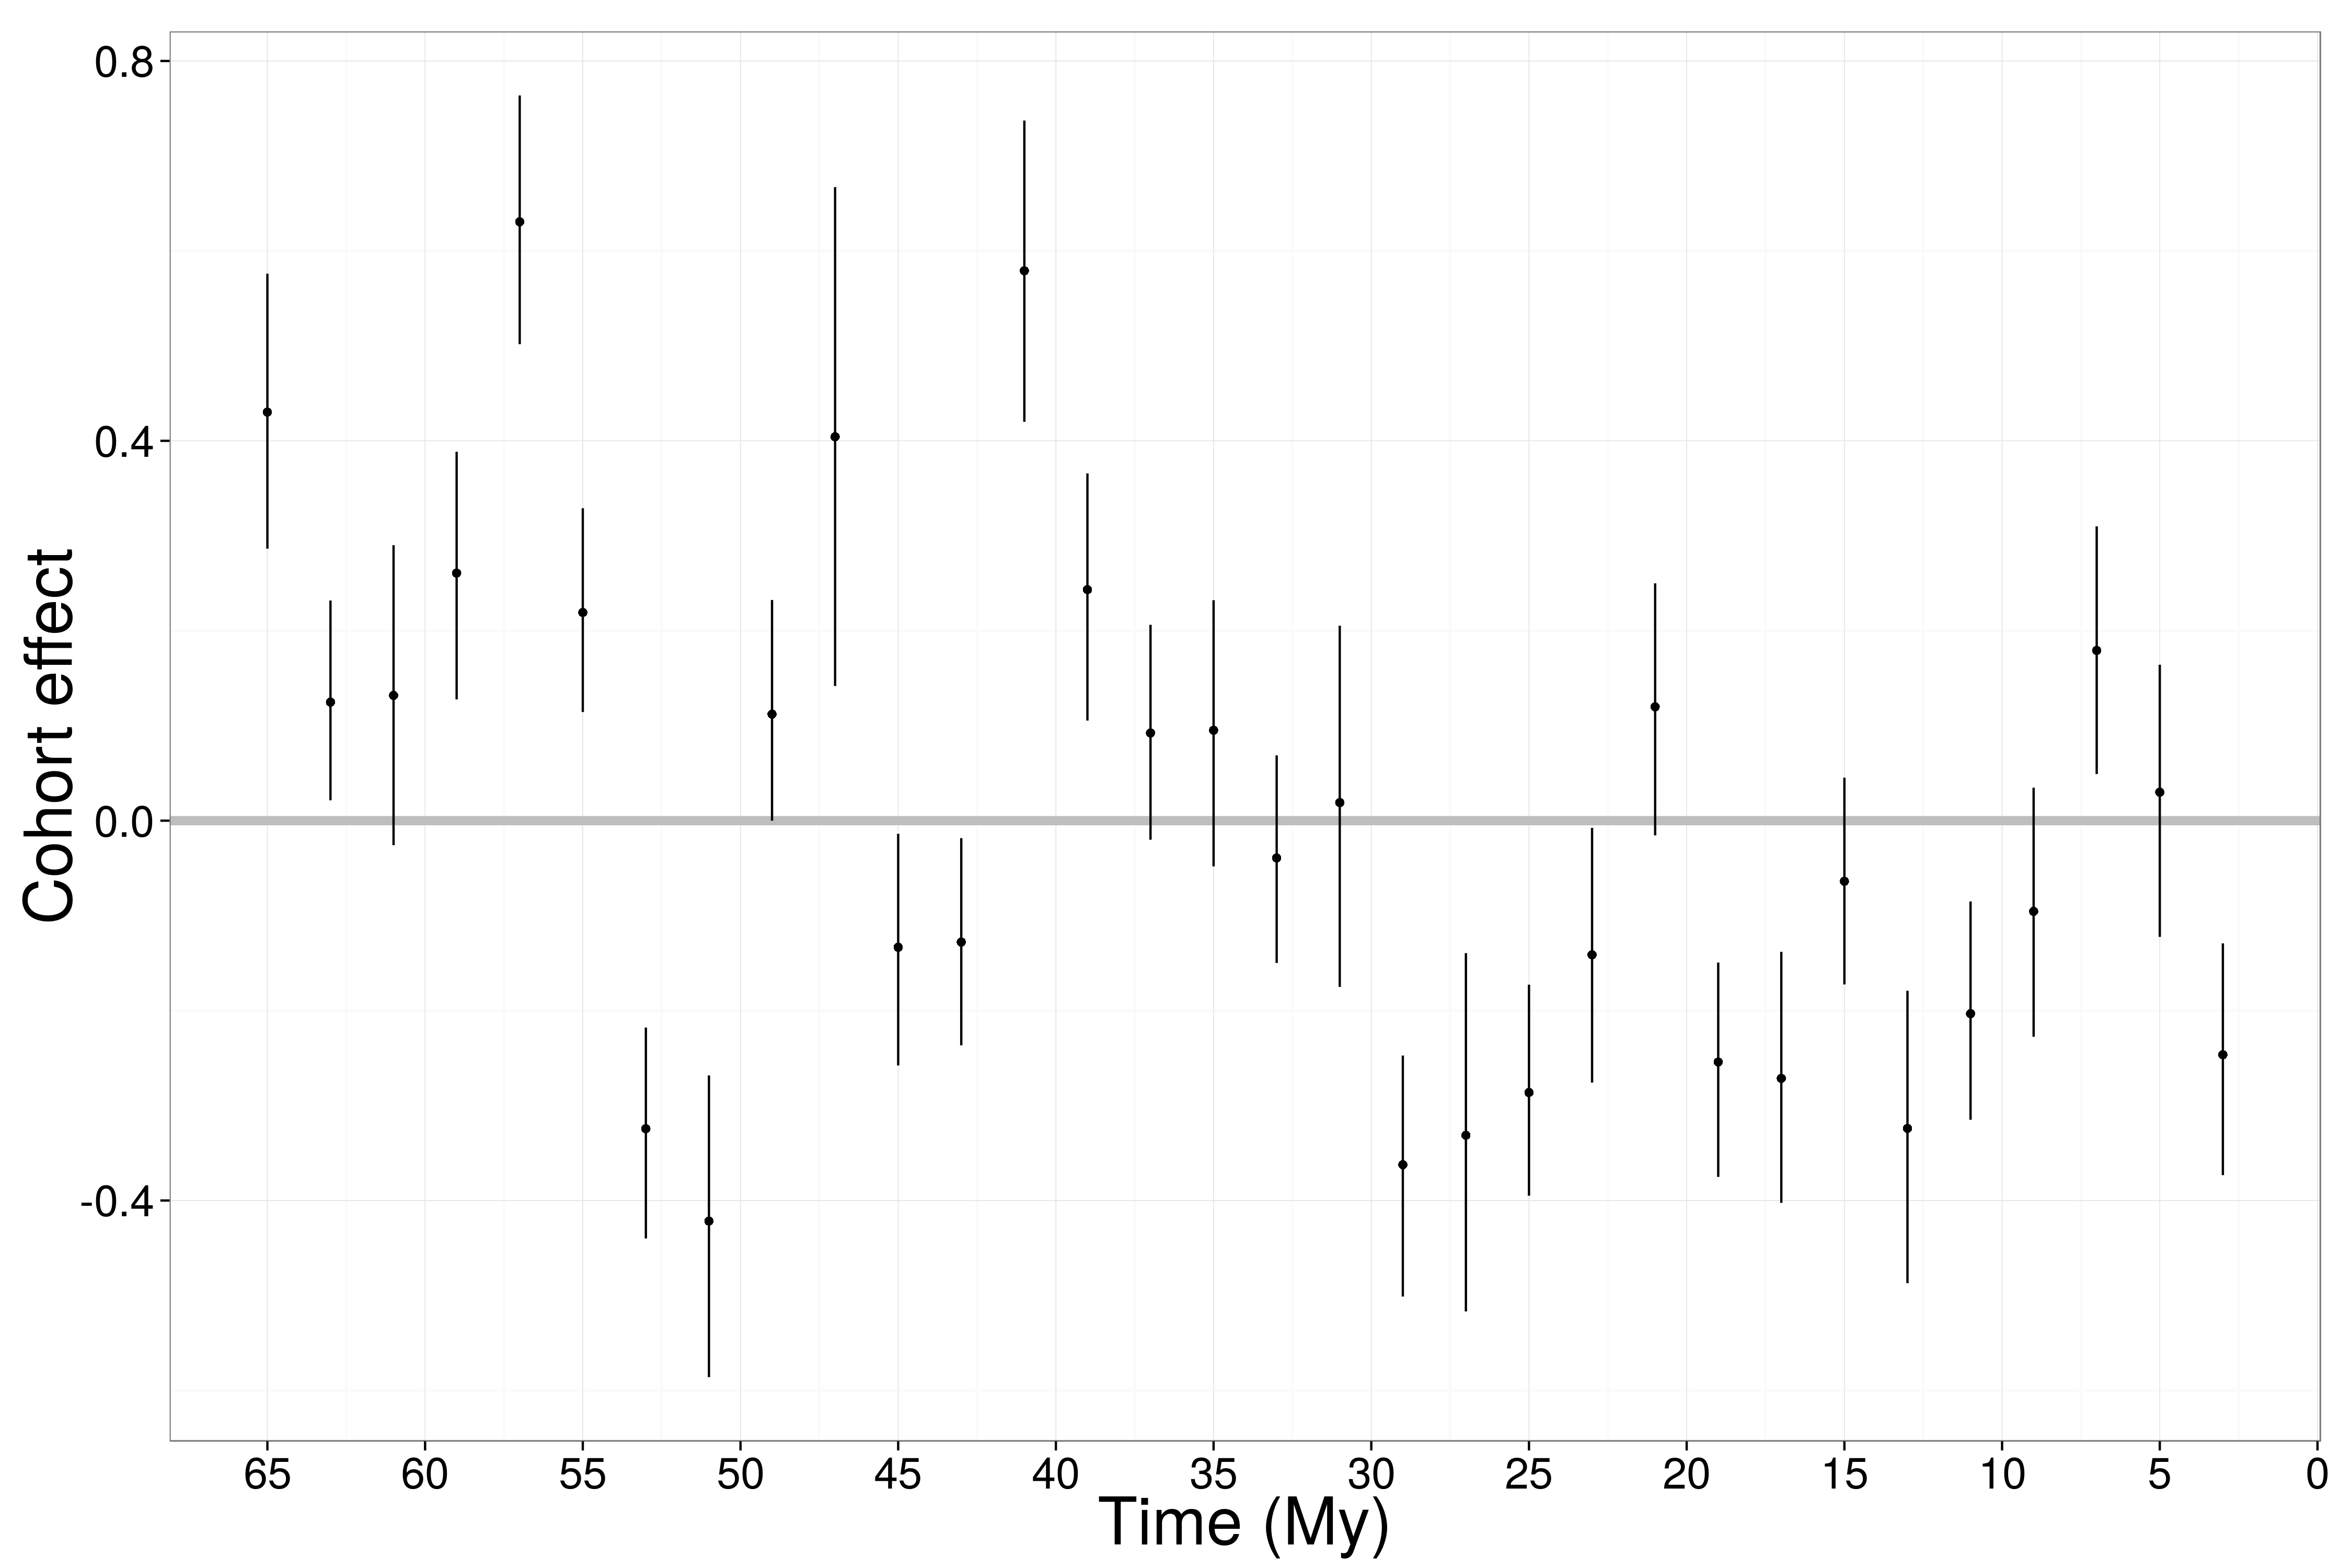
\includegraphics[height = 0.8\textheight, width = \textwidth,  keepaspectratio = true]{figure/cohort_est}
  \end{center}
\end{frame}

\begin{frame}
  \frametitle{Variance partion coefficient}
  \begin{columns}
    \begin{column}{0.5\textwidth}
      \begin{center}
        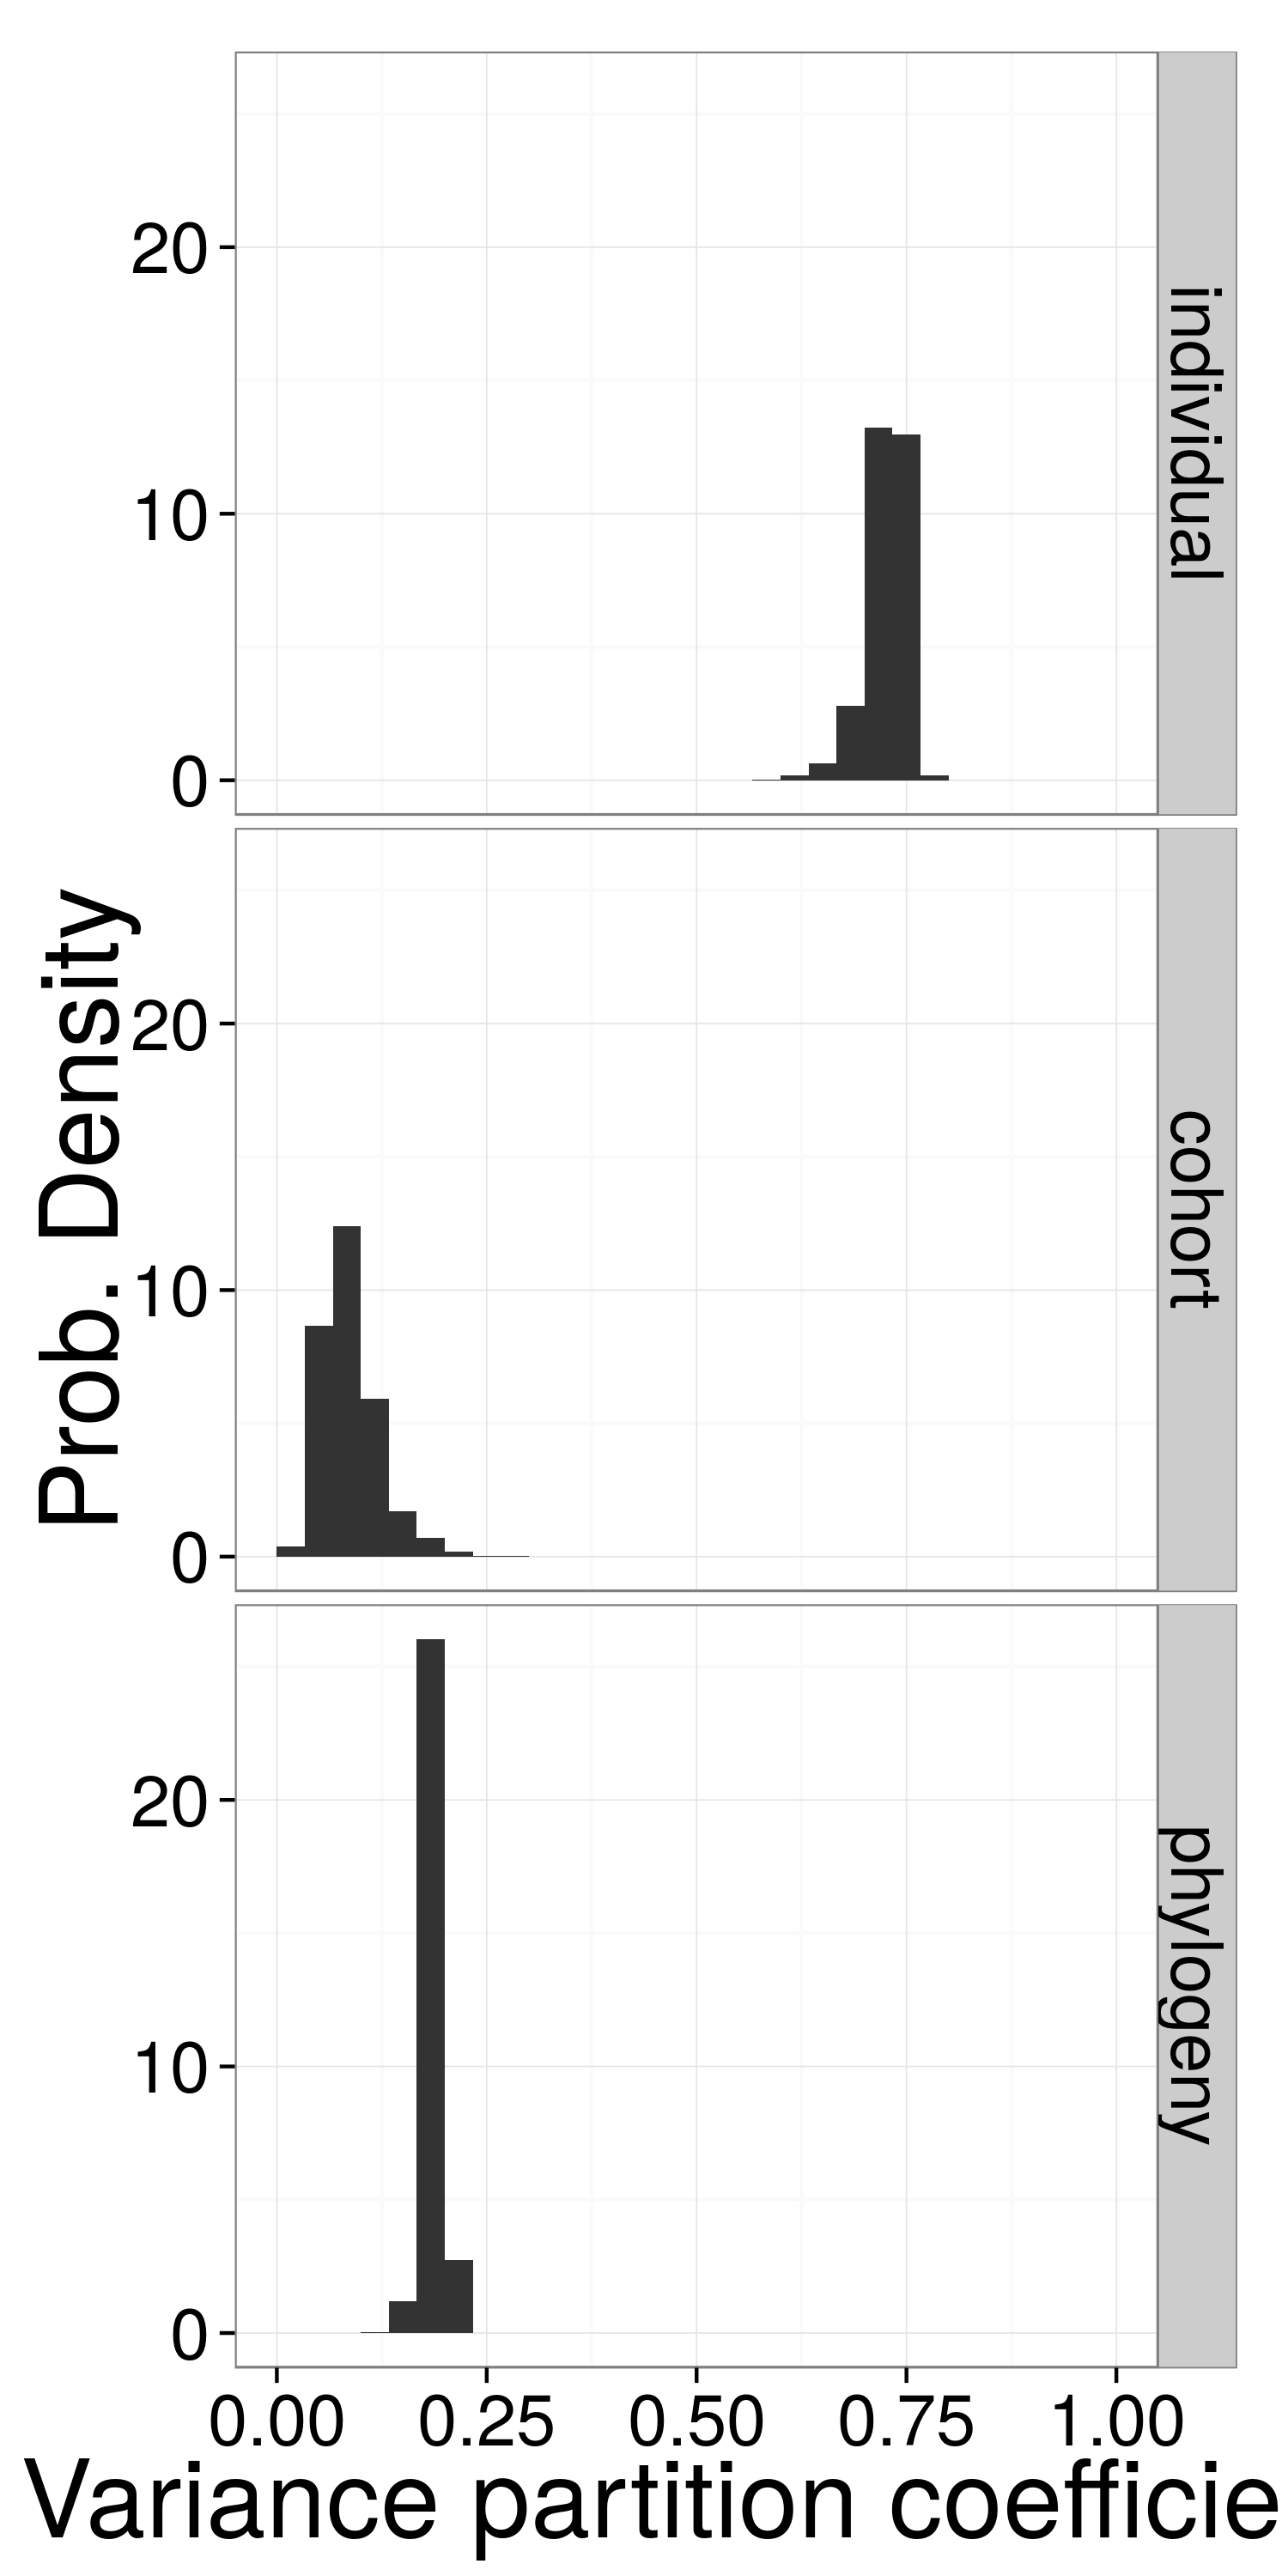
\includegraphics[height = 0.8\textheight, width = \textwidth,  keepaspectratio = true]{figure/variance_est}
      \end{center}
    \end{column}
    \begin{column}{0.5\textwidth}
      \begin{itemize}
        \item Because GLMM, VPC approximated via simulation modified from Goldstein \textit{et al.} '02 \textit{Understanding Statistics}
        \item phylogenetic heritability, \textit{sensu} Lynch '91 \textit{Am. Nat.}, is a special case of VPC.
      \end{itemize}
    \end{column}
  \end{columns}
\end{frame}

\begin{frame}
  \frametitle{Hazard curvature}
  \begin{center}
    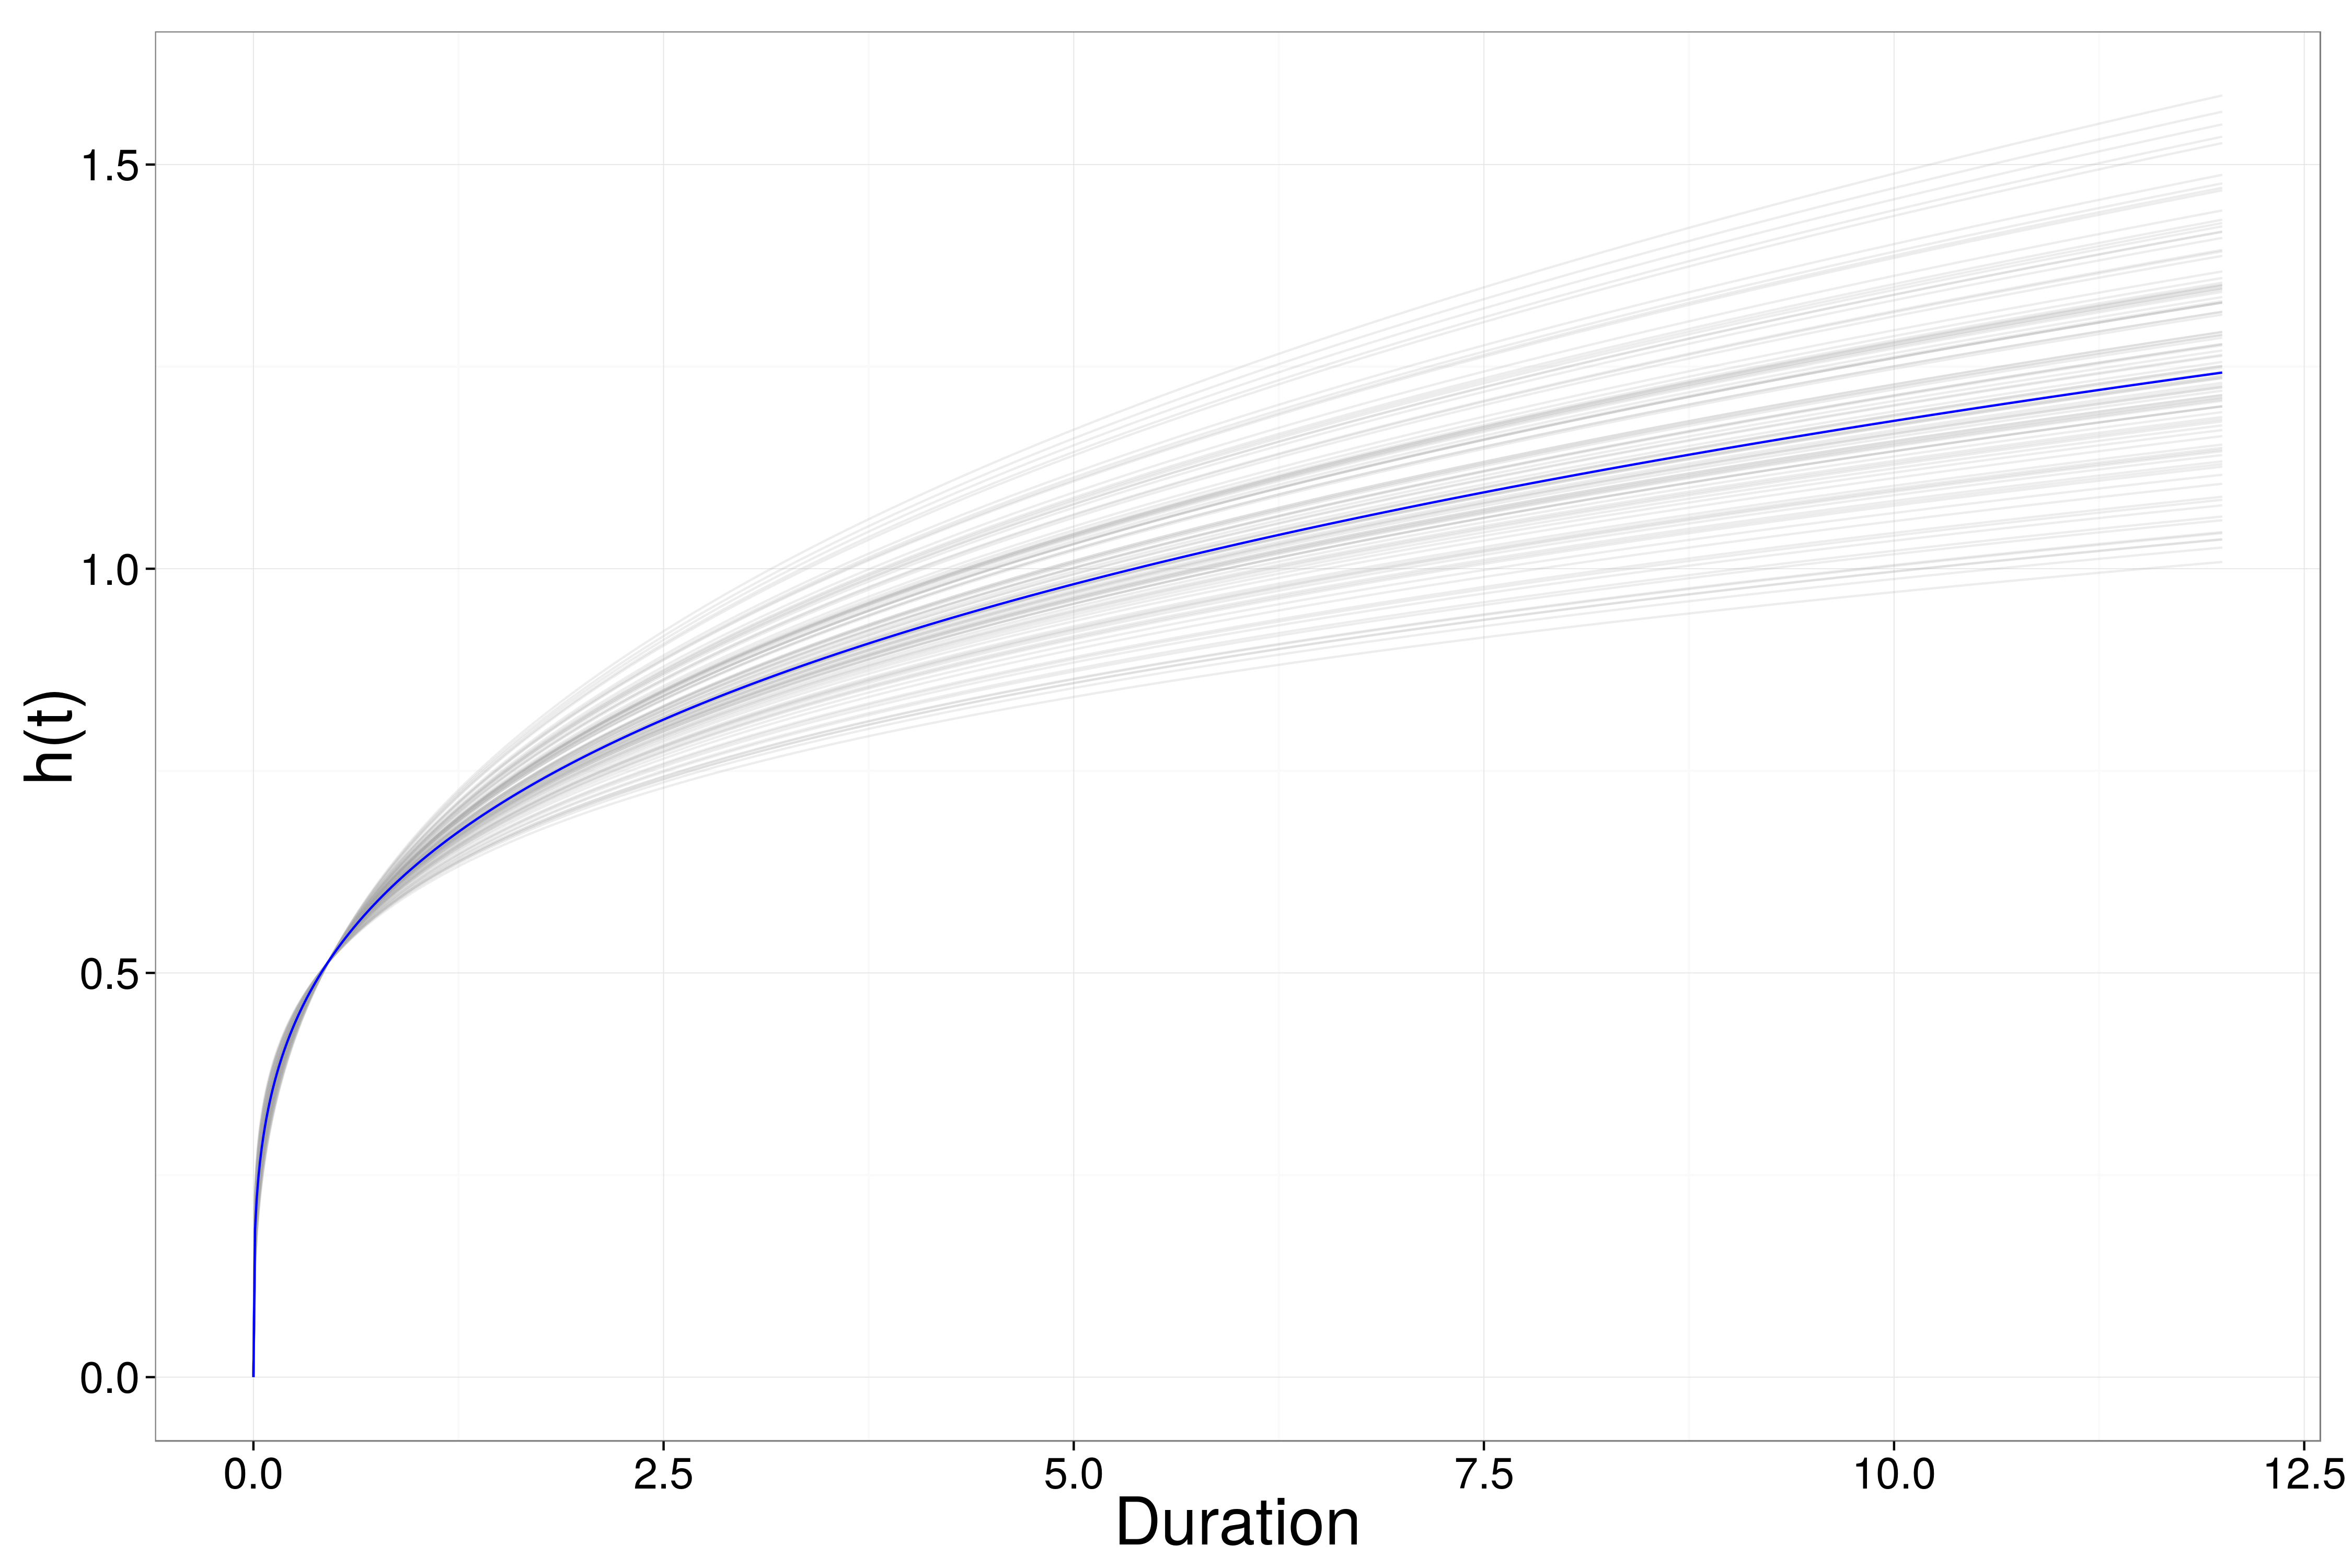
\includegraphics[height = 0.8\textheight, width = \textwidth,  keepaspectratio = true]{figure/haz_est}
  \end{center}
\end{frame}

\begin{frame}
  \frametitle{Meaning}
  \begin{columns}
    \begin{column}{0.5\textwidth}
      Results
      \begin{itemize}
        \item model generally fits; no systematic biases in residuals
        \item comparable probabilistic statements of trait, temporal, and historical effects
          \begin{itemize}
            \item individual level is major source of variance
            \item phylogenetic, cohort effect similar
          \end{itemize}
        \item weak decreasing cohort survival risk over Cenozoic
        \item \(h(t)\) not constant over \(t\), increases slowly
      \end{itemize}
    \end{column}
    \begin{column}{0.5\textwidth}
      Interpretation
      \begin{itemize}
        \item non-zero temporal and historical effects, but very small
          \begin{itemize}
            \item older lineages out-competed by younger (Wagner and Estabrook '14 \textit{PNAS})
          \end{itemize}
        \item increasing extinction with group age (Quental and Marshall '13 \textit{Science})
        \item background extinction; no single mode of extinction
        \item relative effect of universality of covariate, levels of selection(?)
      \end{itemize}
    \end{column}
  \end{columns}
\end{frame}


\begin{frame}
  A model of biological, spatial, and phylogenic effects on Cenozoic mammal co-occurrence
\end{frame}

\begin{frame}
  \frametitle{Biogeographic network}
  \begin{center}
    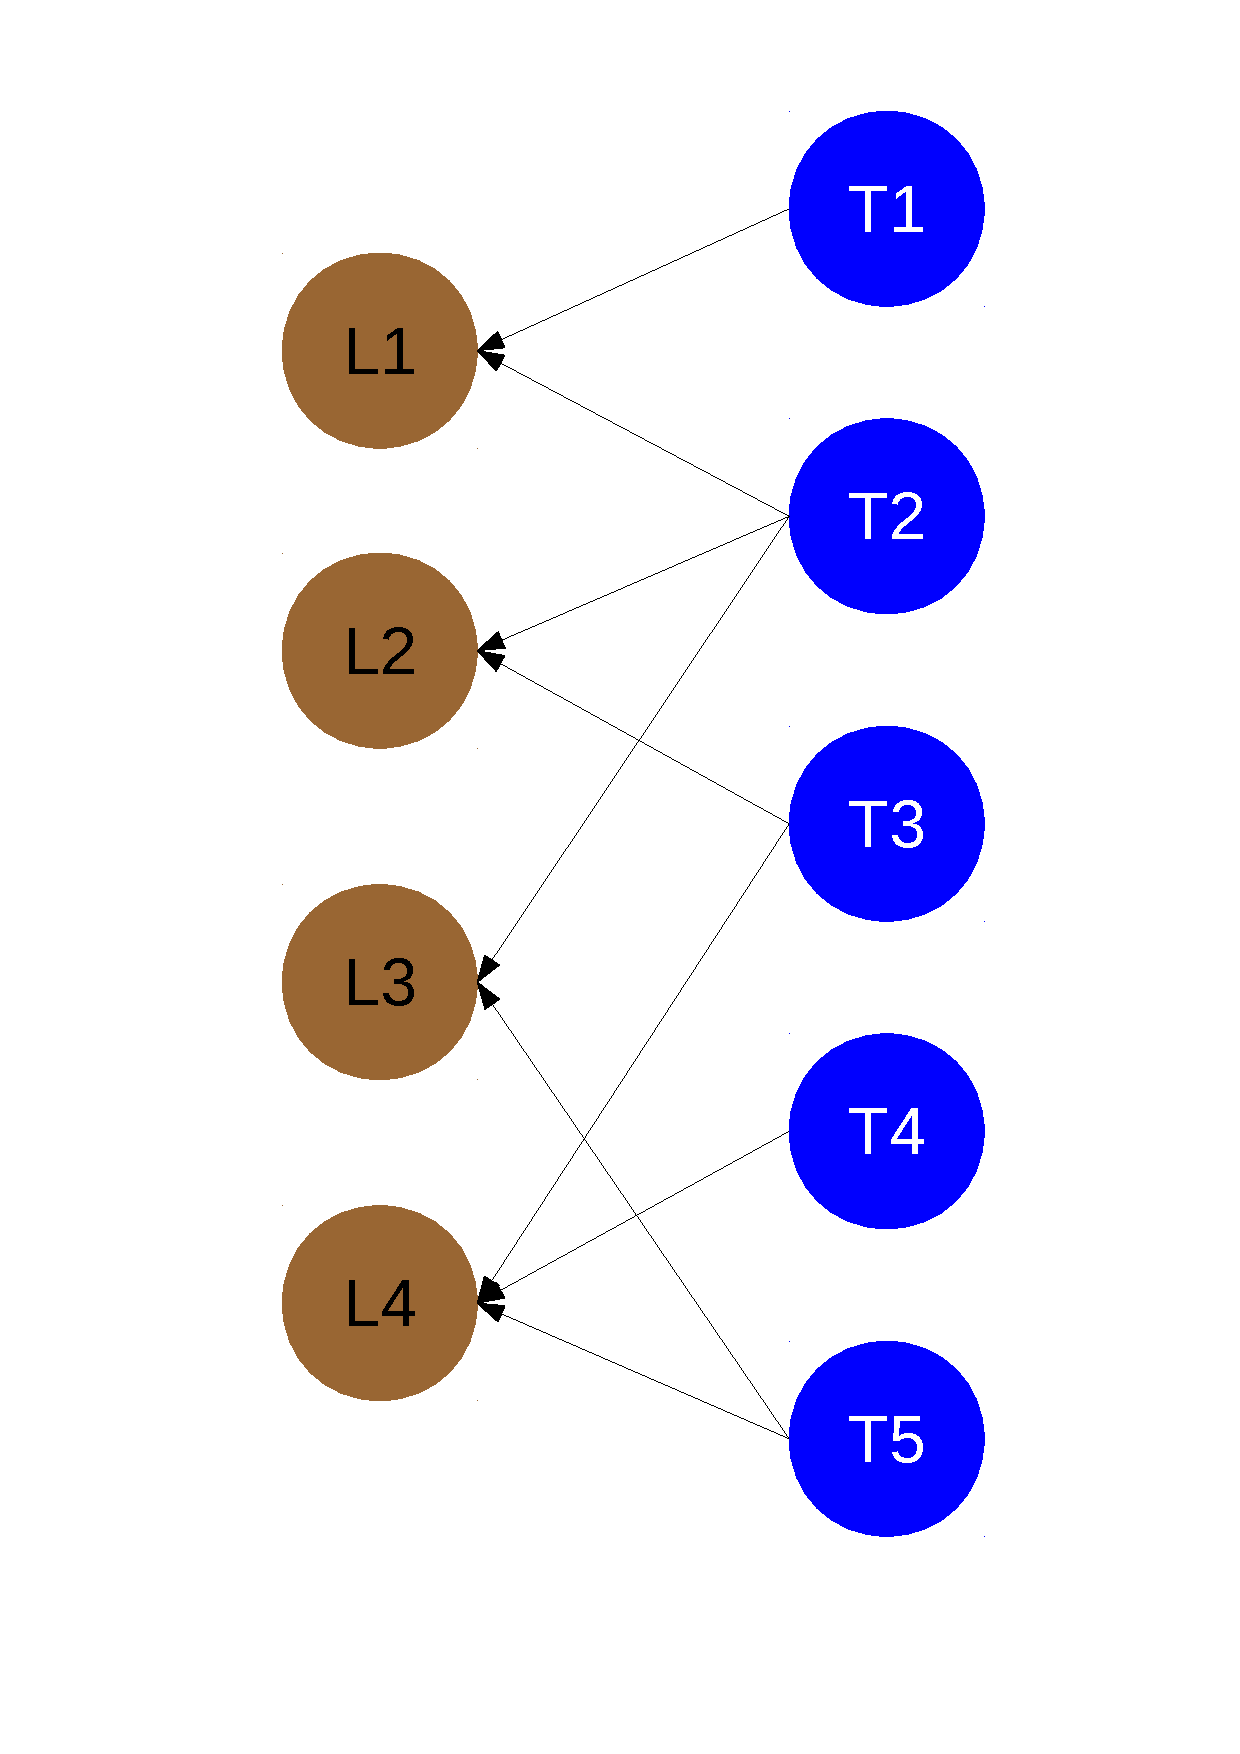
\includegraphics[height = 0.8\textheight, width = \textwidth,  keepaspectratio = true]{figure/bipartite_graph}
  \end{center}
\end{frame}

\begin{frame}
  \frametitle{Species adjacency}
  \begin{center}
    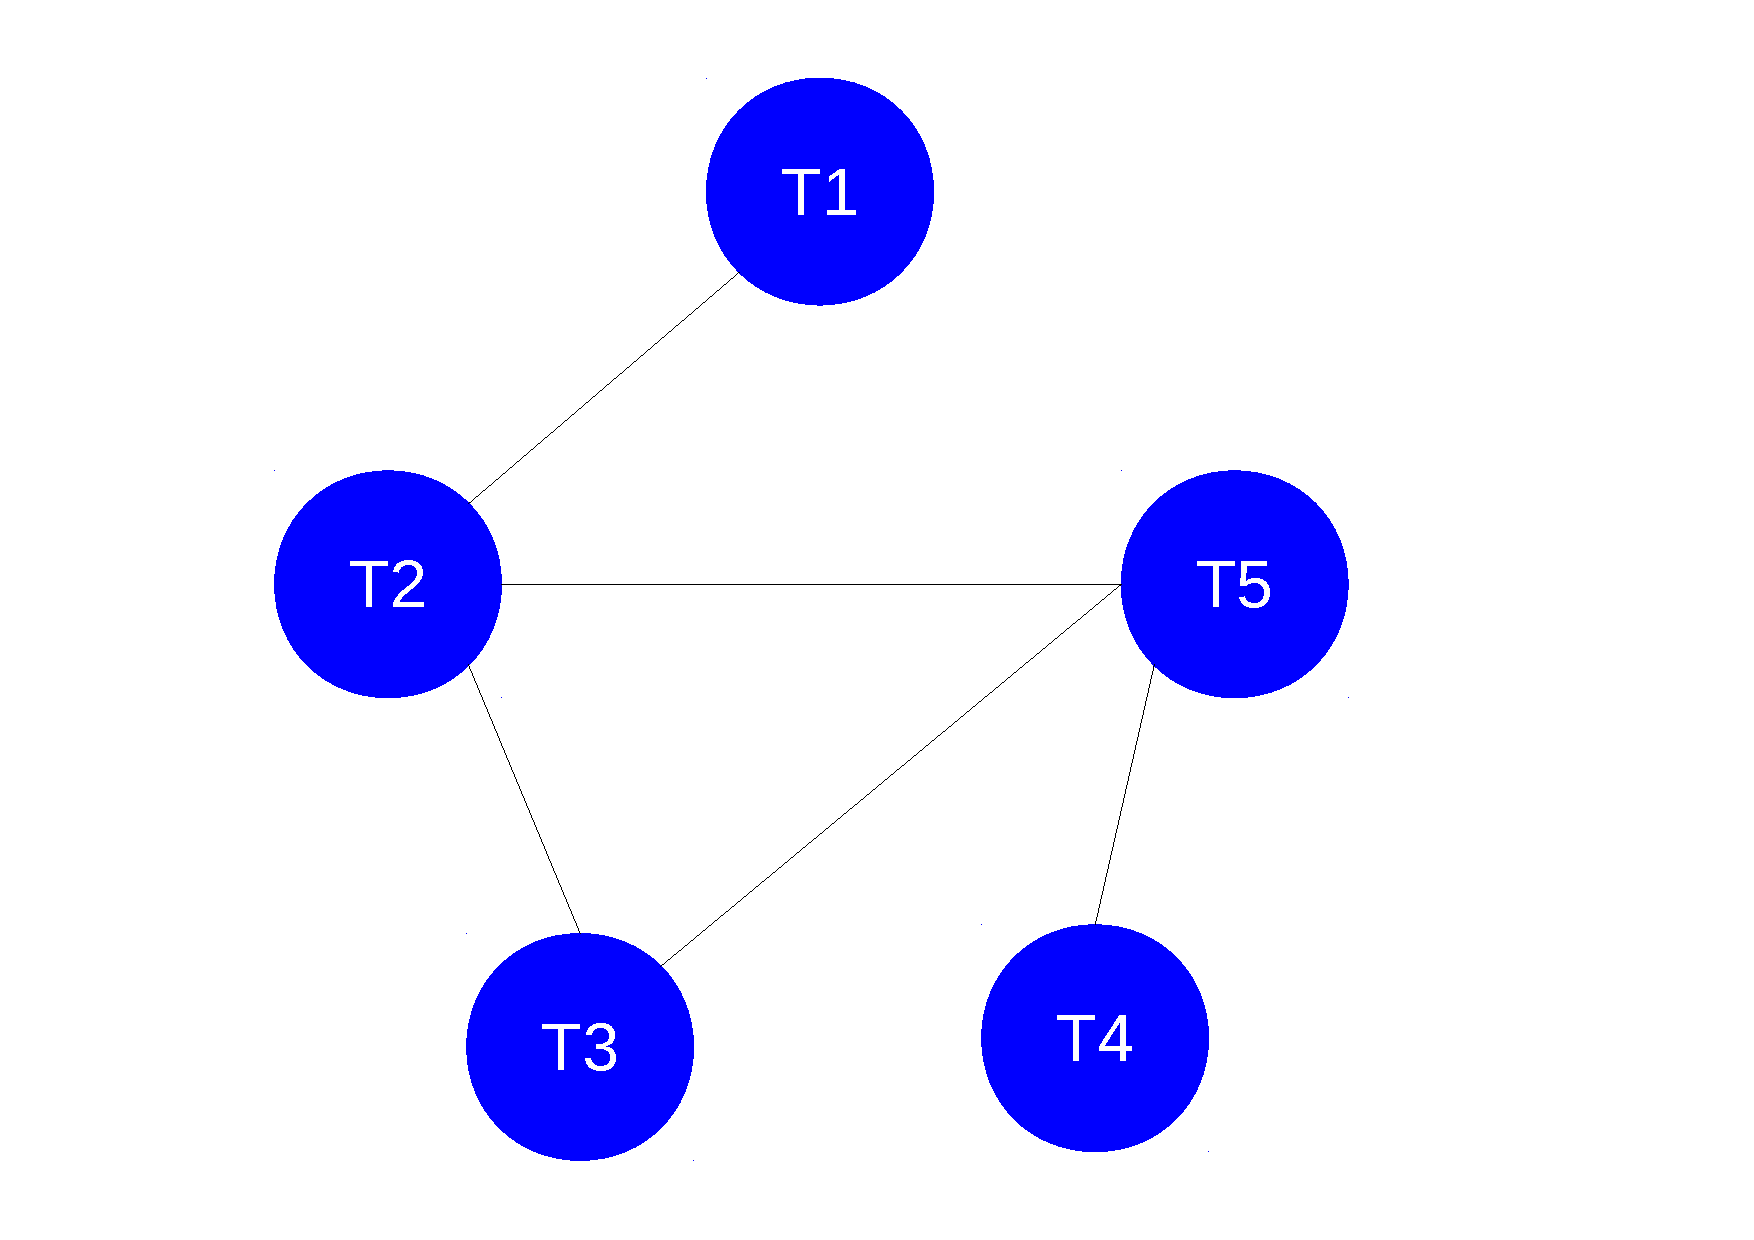
\includegraphics[height = 0.8\textheight, width = \textwidth,  keepaspectratio = true]{figure/one_mode}
  \end{center}
\end{frame}

\begin{frame}
  \frametitle{Autoregressive model}

  Adjacency is also a symmetric n by n matrix, A, with ones on the off-diagonals if the species co-occur.

  CAR prior. Estimate spatial correlation (p) and hierarchical variance variance (sigmasq) as a multivariate normal effect with mean vector all 0 and covariance matrix = sigmasq * (I - p * A)
\end{frame}

\begin{frame}
  \frametitle{Erdos-Renyi graph \(G(n, p)\)}
  \begin{center}
    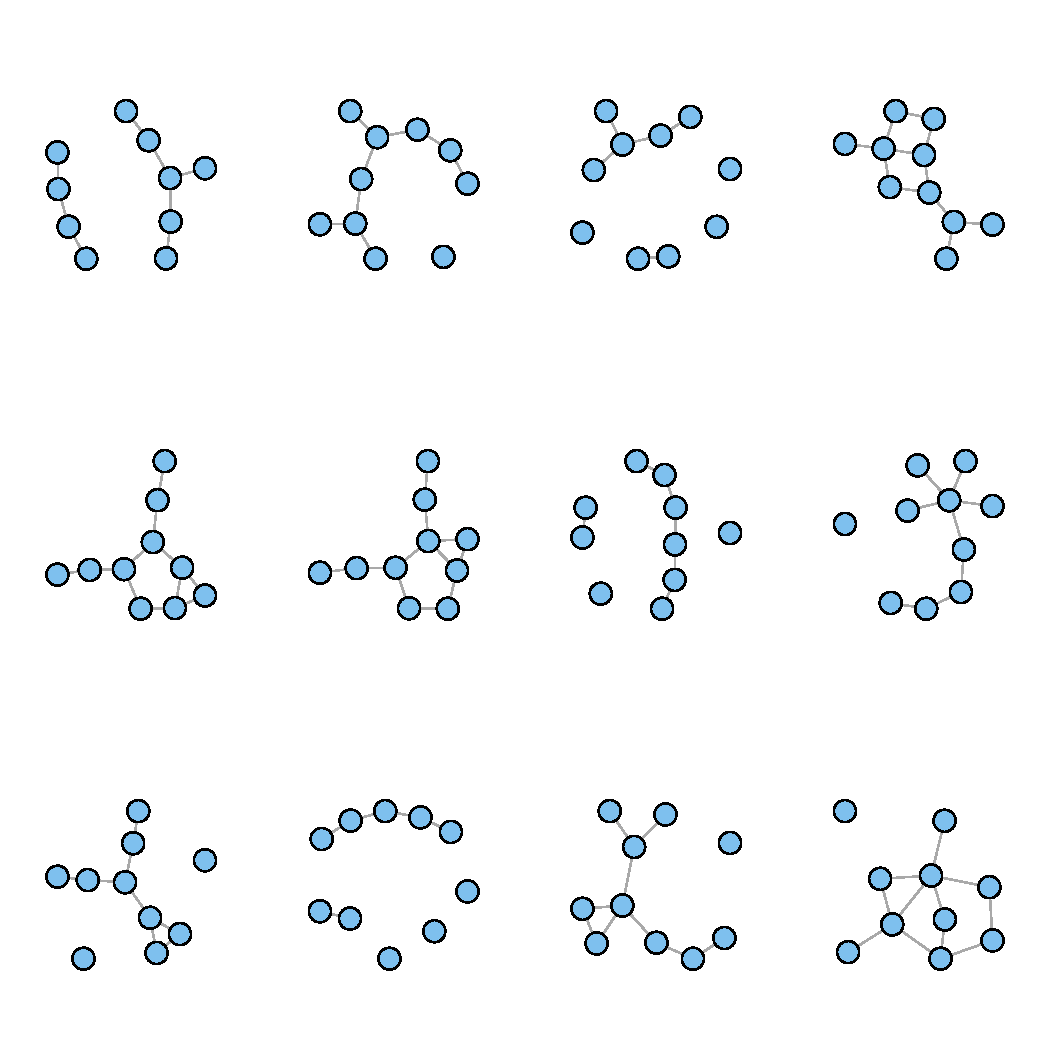
\includegraphics[height = 0.8\textheight, width = \textwidth,  keepaspectratio = true]{figure/rng_graphs}
  \end{center}
\end{frame}

\begin{frame}
  \frametitle{Overdispersion model}

  \begin{block}{Negative Binomial}
    \begin{align*}
      \mathrm{NegBinom}(y | \alpha, \beta) &= {y + \alpha -1 \choose \alpha - 1} \left(\frac{\beta}{\beta + 1}\right)^{2} \left(\frac{1}{\beta + 1}\right)^{y} \\
      \mathrm{reparameterized} \\
      \mathrm{NegBinom}(y | \mu, \phi) &= {y + \phi -1 \choose y} \left(\frac{\mu}{\mu + \phi}\right)^{y} \left(\frac{\phi}{\mu + \phi}\right)^{\phi}
    \end{align*}
  \end{block}
\end{frame}

\begin{frame}
  \frametitle{Model diagram}
  \begin{center}
    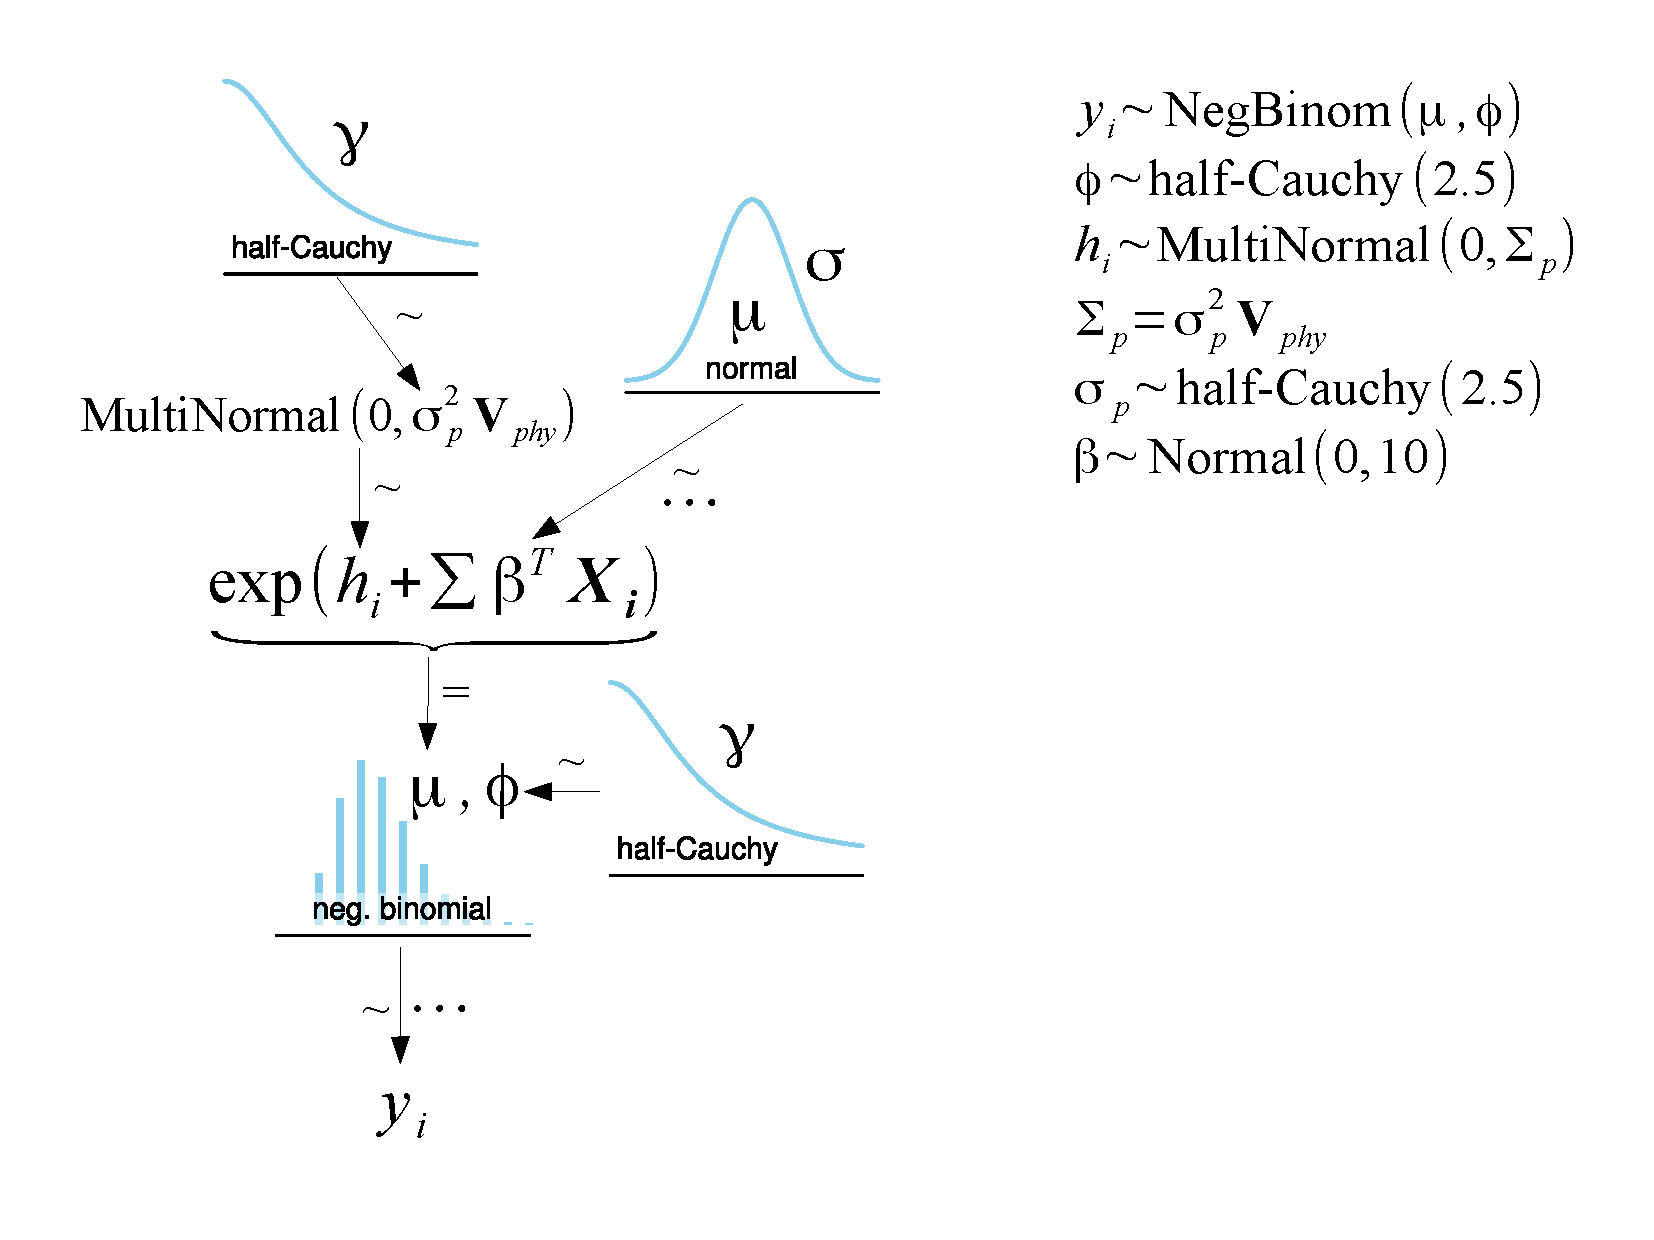
\includegraphics[height = 0.8\textheight, width = \textwidth,  keepaspectratio = true]{figure/mammal_deg_over_model}
  \end{center}
\end{frame}

\begin{frame}
  \frametitle{Analysis framework}
  \begin{center}
    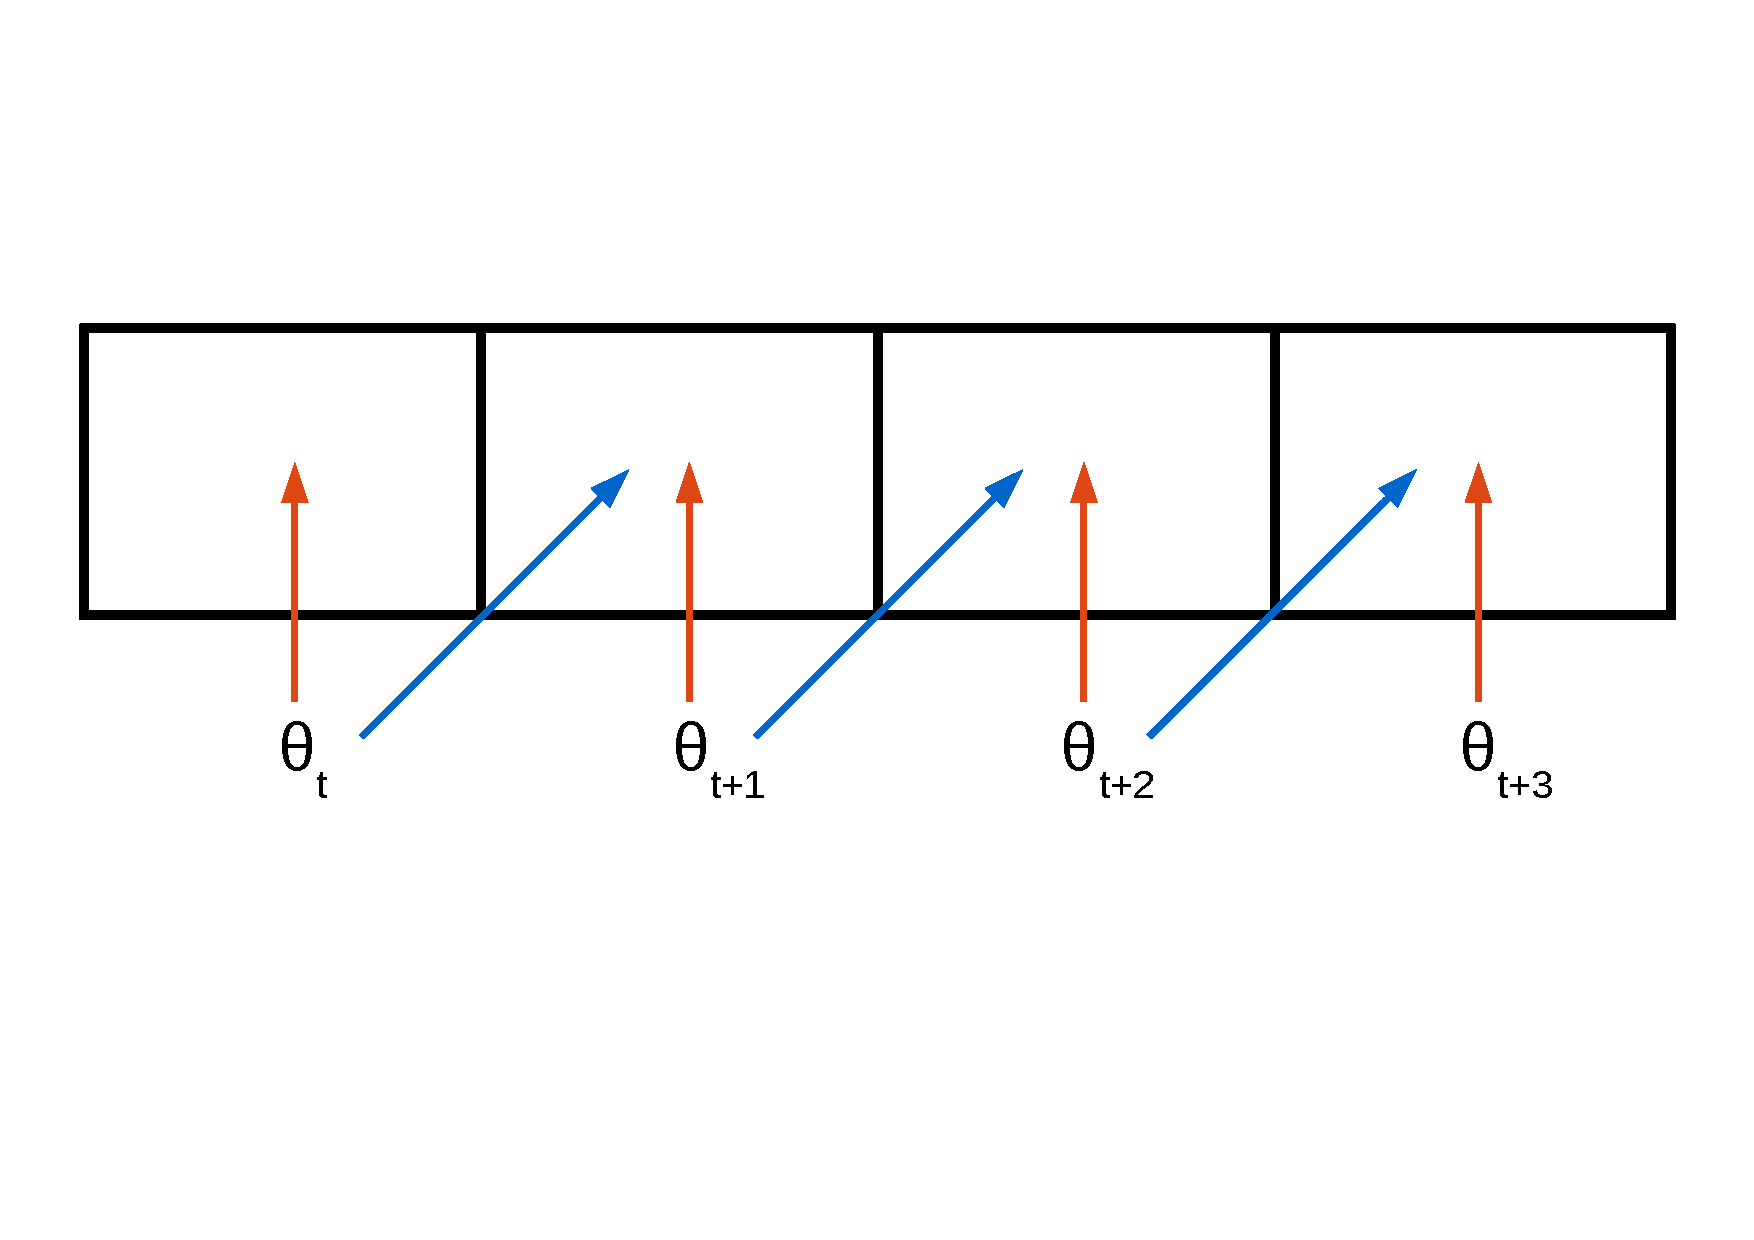
\includegraphics[height = 0.8\textheight, width = \textwidth,  keepaspectratio = true]{figure/predict_perform}
  \end{center}
\end{frame}

% Do I want to try and show some results?


\end{document}
